\documentclass{article}
\usepackage{listings}
\usepackage{enumitem}
\usepackage{amsfonts}
\usepackage{pgfplots}
\usepackage[utf8]{inputenc}
\usepackage{amsmath}
\usepackage{centernot}
\usepackage{amsfonts}
\usepackage{amssymb}
\usepackage{qtree}
\usepackage{fancyhdr}
\usepackage{tikz}
\usepackage{bm}
\usepackage{graphicx}
\usepackage{bbm}
\usepackage[onehalfspacing]{setspace}
\usepackage[margin=0.8in]{geometry} % set margins
\usepackage{biblatex}
\usepackage{multirow}
\usepackage{array}
\usepackage[hidelinks]{hyperref}
\newcolumntype{L}{>{$}c<{$}} % math-mode columns for table
\pgfplotsset{compat=1.18}
\pgfplotsset{width=10cm}

\begin{document}

%\begin{figure}[h!]
%\includegraphics[width=0.4\textwidth]{Lec 5 Img 1}
%\end{figure}

\begin{titlepage}
    \centering

    \vspace*{2cm}

    {\LARGE\bfseries Ensemble Factor Investing with Dynamic Base Model Reweighting\par}

    \vspace{2cm}

    {\large
    Will Ratelband\\
    Candidate for B.Math, University of Waterloo\\
    \par}

    \vspace{1.5cm}

    {\large
    Personal Project\\
    \par}

    \vfill

    {\large
    August 2026
    \par}

    \vspace{1cm}

\end{titlepage}

\break

\tableofcontents

\newpage

\section{Abstract and Acknowledgements}

In this paper, I design a factor investing strategy using an ensemble factor model approach with dynamically updating base model weights. This strategy contains a 'temperature' parameter that is used to control how selective the strategy is in the process of weighting the three base models. The three base models used in this project are Ordinary Least Squares (OLS), Fama-French 3-Factor (FF3), and Elastic Net (EN). \\

Each temperature parameter determines an individual ensemble investing strategy, All such strategies that were tested performed competitively with all three base models, with relative performance dependent on the level of transaction costs, which were also varied to check robustness. When performance measures were aggregated over datasets and transaction cost regimes, dynamically-reweighted ensemble strategies slightly outperformed the equal-weighted ensemble in terms of Sharpe ratio but produced marginally higher turnover.\\

Disclaimer: This is an independent personal project using a University of Toronto Master's of Mathematical Finance, Operations Research course project paper - Shao, J. (V), Miao, X. (A), Zhang, Y. (J), Li, X. (S) -  as inspiration. I have not attended the University of Toronto Master's of Mathematical Finance program and I will not submit this work for credit. All sources, including the Operations Research paper by Shao, J. (V), Miao, X. (A), Zhang, Y. (J), Li, X. (S) and personal communication/informal supervision by Shao, J. (V), are cited.\\

A very big thank you to Shao, J. (V) for her contributions and advice on this project. These were invaluable in gaining a deeper understanding of the ensemble investing strategy rationale as well as the methodology.\\

\break

\section{Introduction}
This project aims to address the question "What are the performance benefits of using dynamically updating base model weights in an ensemble factor model strategy?". These performance benefits are assessed in terms of Sharpe ratio and average portfolio turnover over three datasets, and compared between the equal-weighted ensemble strategy and the dynamically-reweighted ensemble strategies. \\

All strategies are applied to a universe of 10 stocks for an initial estimation window of 60 months. The strategy begins investing after the initial 60-month estimation window. During the first three six-month holding periods, the three base models receive equal ensemble weights. After 18 months of realized out-of-sample prediction errors become available, model weights are dynamically updated according to the softmax transformation of the historical prediction-error measure. It is rebalanced every 6 months using the previous rolling window of 60 months' data until the 132-month mark, at which point performance measures are recorded.\\

\vspace{5mm}

\begin{tabular}{|L|L|}
\hline
\textbf{Months} & \textbf{Phase}\\
\hline
\text{1-60} & \text{Initial rolling window for model estimation}\\
\hline
\text{61-78} & \text{Portfolio is live with equal $\frac{1}{3}$ base model weights. Out of sample mean vector estimate errors are computed}\\
\hline
\text{79-132} & \text{Dynamic base-model reweighting and model re-estimation every six months}\\
\hline
\end{tabular}

\vspace{5mm}

We use the general formula for a linear model to model excess returns: For a time $t = 1,...,T$, $y_{i}^{(t)} = \alpha _i + \beta_{1,i}^{(t)}F^{(t)}_1 + ... + \beta_{K,i}F_{K,t} + \epsilon_i$, where $y_{i,t} = r_i - r_f$, where $r_i$ is the absolute return of the $i^{th}$ asset (given by $\frac{P_{i,t+1}}{P_i,t} - 1$, $r_{f,t}$ is the estimated return of the risk-free asset during the same period.\\

Notation note: Times will be given in superscripts, and the order of subscripts will be factor, asset. For example, the factor loading of the $i^{th}$ asset on the $k^{th}$ factor, at time $t$, is given by $\beta^{(t)}_{k,i}$.\\

We also denote the number of factors by $K$, the number of assets by $N$, and the number of time points incorporated into each rebalancing as $T$. Due to the issue of identical mean vectors (mentioned in Corrections section for now), we use the historical factor mean vector $\bar{F}$ over the last $T_M = 0.6 \cdot T = 36$ months.\\

The paper covers each of the models used, gives some model history (?), outlines the motivation for incorporation into the joint factor model, and explains the process of computing the expected returns and covariance matrix once the factor loadings ($\beta$) are computed. Finally, the computational costs and potential model drawbacks are also presented.\\

\textbf{Data}\\

We have two streams of data as input:\\

1) Asset Prices (for each asset $i$, source: Yahoo Finance):\\

$\{P_i^{(0)}, ...., P_i^{(T)} \}$ from which we compute the asset returns:\\

$r_i^{(1)}, ..., r_i^{(T)}$ where $r_i^{(t)} = \frac{P_i^{(t+1)}}{P_i^{(t)}} - 1$.\\

2) Factor returns (common for use in each asset's analysis, source: Kenneth French Library):\\

There are 8 factors: \\

For each of these factors $k = 1,...,8$, and for each rebalancing period $1, ..., T$, we have the data $\{F_k^{(1)},...,F_k^{(T)}\}$.\\

\vspace{5mm}

\textbf{Backtest Timelines:}\\

\begin{tabular}{|L|L|L|L|}
\hline
\textbf{Dataset} & \textbf{Initial Rolling Window} & \textbf{Portfolio Live + Equal Weighted} & \textbf{Dynamic Base Model Reweighting with 6-month Rebalance}\\
\hline
1 & 1993/01 - 1997/12 & 1998/01 - 1999/06 & 1999/07 - 2003/12\\
\hline
2 & 2004/01 - 2008/12 & 2009/01 - 2010/06 & 2010/07 - 2014/12\\
\hline
3 & 2015/01 - 2019/12 & 2020/01 - 2021/06 & 2021/07 - 2025/12\\
\hline
\end{tabular}\\

\vspace{5mm}

\textbf{Factor Returns Considered:}\\

\begin{tabular}{|L|L|}
\hline
\textbf{Factor} & \textbf{Description}\\
\hline
\text{Mkt-RF} & \text{Market Excess Return: Value-weighted US stocks - one-month Treasury bill rate}\\
\hline
\text{SMB} & \text{Small Minus Big: Return on small cap stocks - return on large cap stocks}\\
\hline
\text{HML} & \text{High Minus Low: Return on high Book-to-Market stocks - return on low Book-to-Market stocks}\\
\hline
\text{RMW} & \text{Robust Minus Weak: Returns on firms with high operating profitability - returns on firms with low operating profitability}\\
\hline
\text{CMA} & \text{Conservative Minus Aggressive: Returns on firms with conservative investment policies - firms with aggressive asset growth}\\
\hline
\text{Mom} & \text{Momentum: Return on stocks with high prior returns - stocks with low prior returns}\\
\hline
\text{ST-Rev} & \text{Short-term reversal: The returns on stocks with low returns in preceding previous month - stocks with high returns in that month}\\
\hline
\text{LT-Rev} & \text{Long-term reversal: The returns on stocks with low long-term prior returns minus stocks with high long-term prior returns}\\
\hline
\end{tabular}\\

\vspace{5mm}

\textbf{Stocks:}\\
Apple (AAPL)\\
Microsoft (MSFT)\\
JPMorgan Chase (JPM)\\
Exxon Mobil (XOM)\\
Johnson and Johnson (JNJ)\\
Walmart (WMT)\\
Coca-Cola (KO)\\
Procter and Gamble (PG)\\
Caterpillar (CAT)\\
IBM (IBM)\\


\break



\section{Ordinary Least Squares (OLS)}

\textbf{3.1: Introduction}\\

The first model used is Ordinary Least Squares (OLS). The returns in excess of the riskfree rate for a given time $t$, $y_i^{(t)} = r_i^{(t)} - r_f^{(t)}$, are modelled as the linear combination of all factors $F_k, k=1,...,K$, plus an intercept $\alpha_i^{(t)}$ and an error term $\epsilon_i^{(t)}$. Note that the error terms (residuals) $\epsilon_i^{(t)}$ are assumed to be uncorrelated with the factor returns $F_i^{(t)}$ for all assets $i = 1,...,N$.\\

$\bm{y_i} = \bm{\alpha_i} + \sum_{k=1}^K \beta_{k,i}^{(t)} F^{(t)}_k + \bm{\epsilon_i}$ \hfill (1)\\

where $\epsilon_i^{(t)}$ is assumed to be normally distributed with zero mean. \\

We can also write this model form as a matrix equation by defining a matrix of factor returns:\\

$\bm{y_i} = X\bm{\beta_i} + \bm{\epsilon_i},$\\

where $X := \begin{pmatrix} 1 & F_1^{(1)} & .... & F_K^{(1)} \\
1 & F_1^{(2)} & ... & F_K^{(2)}\\
... & ... & ... & ...\\
1 & F_1^{(T)} & ... & F_K^{(T)} \end{pmatrix} \in \mathbb{R}^{T \times K + 1}$ and $\bm{\epsilon_i} := \begin{pmatrix}
\epsilon_i^{(1)}\\
...\\
\epsilon_i^{(T)} \end{pmatrix}$ $= \begin{pmatrix} y_i^{(1)} - \hat{y}_i^{(1)}\\
...\\
y_i^{(T)} - \hat{y}_i^{(T)} \end{pmatrix}$\\

\vspace{5mm}

\textbf{3.2: Calculation of $\beta_i$}\\  

We wish to calculate the vector of optimal factor weightings, $\beta_i$, at each rebalancing point of the strategy (eg. every six months). The model uses all factors and assigns a factor loading for each asset $i$ to each factor $F_k$, $\beta_{k,i}^{(t)}$ to minimize the objective function\\

$L(\beta_i) = \|y_i - X\beta_i\|_2^2$\\

$\Rightarrow \hat{\beta}_i^{(t)} = \underset{\beta_i}{\text{argmin}} \|y_i - X\beta_i\|_2^2$\\

Expanding, we obtain:\\

$\|y_i - X\beta_i\|_2^2 = (y_i - X\beta_i)^T(y_i - X\beta_i)$\\

$= y_i^Ty_i - y_i^TX\beta_i - (X\beta_i)^Ty_i + (X\beta_i)^TX\beta_i$\\

$= y_i^Ty_i -y_i^TX\beta_i - y_i^TX\beta_i - \beta_i^TX^TX\beta_i$\\

$= y_i^Ty_i - 2y_i^TX\beta_i + \beta_i^TX^TX\beta_i$\\

$\Rightarrow$ (by differentation rules in linear algebra) $\frac{\partial L(\beta_i)}{\partial \beta_i} = 2X^Ty_i - 2X^TX\beta_i$.\\

Then setting $\frac{\partial L(\beta_i)}{\partial \beta_i} = 0$, we have that: $\beta = (X^TX)^{-1}X^Ty_i$ and this is our OLS factor loading estimate.\\

\vspace{5mm}

\textbf{3.3 Obtaining Mean and Covariance Estimates}\\

Once we have the estimate $\hat{\beta_i^{(t)}} = (X^TX)^{-1}X^Ty_i$, we have expressed each excess return for asset $i$ at each time point $t$ as a linear combination of the eight factor returns:\\

\[ Y_i^{(t)} = \hat{\alpha}_i^{(t)} + \hat{\beta_{1,i}^{(t)}}F_1^{(t)} + ... + \hat{\beta_{K,i}^{(t)}}F_K^{(t)} + \epsilon_i^{(t)} \], where $K=8$.\\

Next, we can obtain the mean vector of returns $\mu = \begin{pmatrix} \mu_1 \\
\mu_2\\
...\\
\mu_N \end{pmatrix} $ using the historical average of each factor return over the training period (previous $T_M=36$ months). We can also obtain the covariance matrix $Q$, where $Q_{i,j} = \text{Cov}(y_i,y_j)$, where we recall each pair $y_i,y_j$.\\

The mean vector is estimated simply by:

\[ \mu_i = \alpha_i + \beta_{1,i}\bar{F_1} + ... + \beta_{K,i}\bar{F_K} \], where $\bar{F} = \frac{1}{T_M}\sum_{t=1}^{T_M} F^{(t)}$ and $\bar{F_k}$ is the $k^{th}$ entry of the vector $\bar{F}$.\\

Denoting $\hat{Y}_i = X\hat{\beta}_i$ for all assets $i$, we have $\text{Cov}(y_i,y_j) = Cov(\hat{Y}_i + \epsilon_i, \hat{Y}_j + \epsilon_j)$\\

\[ \Rightarrow \hat{\text{Cov}}(y_i, y_j) = \text{Cov}(\hat{Y}_i, \hat{Y}_j) + Cov(\epsilon_i,\epsilon_j) \] since we assume the processes $\{F_i^{(t)}\}$ and $\{\epsilon_j^{(t)}\}$ are uncorrelated for all $(i,j) \in \{1,...,N\} \times \{1,...,N\}$.\\

\[= \mathbb{E}[(\hat{Y}_i - \mu_i)(\hat{Y}_j - \mu_j)] + \mathbb{E}[(\hat{\epsilon}_i - \bar{\epsilon}_i)(\hat{\epsilon}_i - \bar{\epsilon}_i)]\]\\

which we estimate using the sample covariance:\\

\[= \frac{1}{T-1} \sum_{t=1}^T [(X_t\hat{\beta_i} - \mu_i)(X_t\hat{\beta_j}-\mu_j)] + \delta_{i,j}\text{Var}(\epsilon_i)\], where $X_t$ is the $t^{th}$ row of the matrix $X$, equivalent to $F^{(t)T}$.\\

\[= \frac{1}{T-1} \sum_{t=1}^T [\beta_i^T(X_t^T - \bar{F}) \cdot (X_t - \bar{F}^T)\beta_i] + \delta_{i,j}\text{Var}(\epsilon_i)\], factoring out $\beta_i^T$ and $\beta_i$.\\

\[= \beta_i^T \frac{1}{T-1} \sum_{i=1}^T (F_t - \bar{F})(F_t - \bar{F})^T \beta_i + \delta_{i,j}\text{Var}(\epsilon_i)\]\\

$\Rightarrow$ defining the matrix $V = \begin{pmatrix} \hat{B}_{1,1} & ... & \hat{B}_{1,N}\\
... & ... & ...\\
\hat{B}_{K,1} & ... & \hat{B}_{K,N} \end{pmatrix}$, (where we note that the $i^{th}$ column of $V$ is $\hat{\beta_i}$, we have that our sample covariance matrix for our asset returns, given our estimate $\hat{\beta}$, is\\

$V^TFV + D$, $F = \hat{Cov}(F^{(t)}) = \frac{1}{T-1}(F^{(t)}-\bar{F})(F^{(t)}-\bar{F})^T$ and $D = \text{Cov}(\epsilon) = 
\begin{pmatrix}
\hat{\sigma}_{\epsilon_1}^2 & 0 & 0 &... & 0\\
0 & \hat{\sigma}_{\epsilon_2}^2 & 0  & ... & 0\\
...\\
0 & 0 &  ... & 0 & \hat{\sigma}_{\epsilon_N}^2 \end{pmatrix}$, since we are assuming the residuals are uncorrelated and therefore $D_{i,j} = \delta_{i,j}\text{Var}(\epsilon_i)$.\\

So, to summarize, we have our estimate of the mean return vector and covariance matrix, estimated at time step $t$ (which will be a rebalancing point for the portfolio in a dataset), given by OLS, as $\mu = \begin{pmatrix} \mu_1\\
...\\
\mu_N \end{pmatrix} = \begin{pmatrix} \hat{\alpha} & V^T \end{pmatrix} \begin{pmatrix} 1\\
\bar{F} \end{pmatrix}$ where we recall $\hat{\alpha} = \begin{pmatrix} \hat{\alpha_1}\\
...\\
\hat{\alpha_N} \end{pmatrix}$ and $\bar{F} = \begin{pmatrix} \frac{1}{T_M} \sum_{\tau=1}^{T_M} F_1^{(\tau)} \\
...\\
\frac{1}{T_M}\sum_{\tau=1}^{T_M} F_K^{(\tau)} \end{pmatrix}$, where $T_M = 0.6 \cdot T = 36$ months.\\

\vspace{5mm}

\textbf{Summary and Rolling Window Implementation}\\

At each sixth month in the data, we implement the above steps to calculate $\hat{\beta}^{(t)}$ using the OLS factor selection method. Once we have $\hat{\beta}^{(t)}$, we calculate the estimated mean return vector $\mu^{(t)}$ using the previous $T_M=36$ months of data. The covariance matrix is estimated as above based on $\hat{\beta}^{(t)}$.\\

The procedure for each of the following two models is similar: using the previous $T=60$ months of data, we calculate the optimal factor loadings $\hat{\beta}^{(t)}$ and use these to find the mean return vector and covariance matrix for that model at each rebalancing point (where we use $T_M = 36$ months of factor returns to calculate the mean return vector for each base model (including OLS).\\

\break

\section{3-Factor Fama-French Model}

\textbf{4.1 Introduction}\\

The next model used is well-grounded in finance and has been extensively empirically tested. The 3-factor Fama-French model incorporates a subset of the original 8 factors, namely MKTRF, SMB, and HML returns. This model extends the traditional CAPM, $y_i = \beta_i(MKT_RF)$, where $y_i$ once again denote the excess return $r_i - r_f$.\\

Since the 3-factor FF model is simply the application of the OLS procedure to a subset of the $K=8$ original factors (MKT-RF, SMB, and HML so $K=3$), the factor loadings $\hat{\beta}^{(t)}$ are obtained in exactly the same way. Note the dimensionality differences:\\

We model each return $y_i = r_i - r_f = X \beta_i + \epsilon_i$ for each asset $i$, where this time, $X = \begin{pmatrix} 1 & F_1^{(1)} & F_2^{(1)} & F_3^{(1)}\\
...\\
1 & F_1^{(T)} & F_2^{(T)} & F_3^{(T)} \end{pmatrix}$ and $\beta_i = \begin{pmatrix} \alpha_i\\
\beta_{1,i}\\
\beta_{2,i}\\
\beta_{3,i} \end{pmatrix}$ (and $T=60$ as before).\\

\vspace{5mm}

\textbf{4.2 $\beta_i$ Calculation}\\

Since this is an OLS application with reduced dimension, considering the new matrices $X$ and using the same notation as in the OLS section (section 3), we once again have $\hat{\beta_i} = (X^TX)^{-1}X^Ty_i$ as our estimate- refer to subsection 3.2: Calculation of $\beta_i$ in the OLS section for the derivation.\\

Once we have $\hat{\beta_i} = \begin{pmatrix} \hat{\alpha_i}\\
\hat{\beta_{1,i}}\\
\hat{\beta_{2,i}}\\
\hat{\beta_{3,i}} \end{pmatrix}$, we can calculate the mean return vector and the covariance matrix in the same way as with OLS (recall FF 3-factor is OLS performed on the $\{$MKT-RF, HML, SMB$\}$ subset of the original eight factors.\\

We have $\mu_{\text{FF3}} = \begin{pmatrix} \mu_1\\
\mu_2\\
...\\
\mu_N \end{pmatrix} = \begin{pmatrix} \hat{\alpha_1} + \hat{\beta_{1,1}} \bar{F}_1 + ... + \hat{\beta_{K,1}} \bar{F}_K\\
...\\
\hat{\alpha_N} + \hat{\beta_{1,N}}\bar{F}_1 + ... + \hat{\beta_{K,N}}\bar{F}_K \end{pmatrix} =\begin{pmatrix} \hat{\alpha} & V^T \end{pmatrix} \begin{pmatrix} 1\\
\bar{F}_{36} \end{pmatrix}$, where we again define the $K \times N$ matrix $V$ as\\

\vspace{3mm}

$V = \begin{pmatrix} \hat{\beta_{1,1}} & ... & \hat{\beta_{1,N}}\\
... & ... & ...\\
\hat{\beta_{K,1}} & ... & \hat{\beta_{K,N}} \end{pmatrix}$.\\

Then our covariance matrix $Q$ is once again given by $Q = V^TFV + D$, where $F = \hat{Cov}(F^{(t)}) = \frac{1}{T-1}(F^{(t)} - \bar{F})(F^{(t)} - \bar{F})^{T}$ and $D = \begin{pmatrix} \hat{\sigma_{\epsilon_1}}^2 & 0 & 0 & ... & 0\\
0 & \hat{\sigma_{\epsilon_2}}^2 & 0 & ... & 0\\
 & & ... & &\\
0 & 0 & ... & 0 & \hat{\sigma_{\epsilon_N}}^2 \end{pmatrix}$. We assume that the residuals are uncorrelated as with the OLS model.\\

Note that in the covariance matrix calculation, $\bar{F}$ uses the full 60 previous months as this is part of the covariance calculation.\\


\break

\section{Elastic Net}

\textbf{5.1 Introduction}\\

Denoting $\beta_i = \begin{pmatrix} \alpha_i\\
\beta_{i-} \end{pmatrix}$, the Elastic Net regression method alters the OLS optimization problem, $\min_{\beta_i} \|X\beta - y\|_2^2 + \lambda_1 \| \beta_{i-} \|_1 + \lambda_2 \| \beta_{i-} \|_2^2$. Prior to being used in the optimization, the factor returns comprising matrix $X$ are standardized to avoid scale dependency among the penalty terms.\\

This regression strategy places a penalty term $\lambda_1$ on the 1-norm of the factor loadings and a penalty term of $\lambda_2$ on the 2-norm of the factor loadings. Note that the intercept $\alpha_i$ is not being penalized.\\

Denoting $\hat{\beta}_i$ as the solution to the above problem, we once again obtain the mean vector $\mu_{EN}$ and covariance matrix $Q_{EN}$ in the same way as with OLS and 3-Factor Fama-French models:\\

$\mu_{EN} = \begin{pmatrix} \hat{\alpha}_{EN} & V^T \end{pmatrix} \begin{pmatrix} 1\\
\bar{F}_{36} \end{pmatrix}$ where we recall $\hat{\alpha_{EN}} = \begin{pmatrix} \hat{\alpha}_1 \\
...\\
\hat{\alpha_N} \end{pmatrix}$ and $\bar{F}_{36} = \begin{pmatrix} \frac{1}{T_M} \sum_{\tau=1}^{T} F_1^{(\tau)}\\
...\\
\frac{1}{T_M} \sum_{\tau=1}^{T_M} F_K^{(\tau)} \end{pmatrix}$, $V = \begin{pmatrix} \hat{\beta_{1,1}} & ... & \hat{\beta_{1,N}}\\
... & ... & ...\\
\hat{\beta_{K,1}} & ... & \hat{\beta_{K,N}} \end{pmatrix}$.\\

$Q_{EN} = V^TFV + D$, where $F = \hat{Cov}(F^{(t)}) = \frac{1}{T-1}(F^{(t)} - \bar{F})(F^{(t)} - \bar{F})^{T}$ and $D = \begin{pmatrix} \hat{\sigma_{\epsilon_1}}^2 & 0 & 0 & ... & 0\\
0 & \hat{\sigma_{\epsilon_2}}^2 & 0 & ... & 0\\
 & & ... & &\\
0 & 0 & ... & 0 & \hat{\sigma_{\epsilon_N}}^2 \end{pmatrix}$. We again assume that the residuals are uncorrelated as with the OLS and 3-Factor Fama French models.\\

The Elastic Net model is implemented using the same rolling window as OLS and 3-Factor Fama French.\\

\textbf{5.2 $\lambda_1$ and $\lambda_2$ Selection}\\

The parameters $\lambda_1$ and $\lambda_2$ were selected using a 4-fold chronological validation to select optimal parameters while avoiding lookahead bias. The folds were selected as follows:\\

Fold 1 times: $\{0,36,42\}$- Training window 0-36 months, validation window 36-42 months.\\

Fold 2 times: $\{6,42,48\}$- Training window 6-42 months, validation window months 42-48 months.\\

Fold 3 times $\{12,48,54\}$- Training window 12-48 months, validation window months 48-60.\\

Fold 4 times $\{18,54,60\}$- Training window 18-54 months, validation window months 54-60.\\

\break

\section{Ensemble Step}

\vspace{5mm}

This project aims to harness the benefits of an ensemble strategy to estimate the mean returns and covariance matrix of the ten assets, but also aims to take advantage of base models that have a strong recent history of predicting the mean return vector.\\

The base weights for the ensemble covariance matrix estimate are kept constant at $\{\frac{1}{3}, \frac{1}{3}, \frac{1}{3}\}$ to accentuate the differences in the mean return vector estimates of the base models.\\

The approach adopted into this paper is to combine the base model estimates of the mean return vector using dynamically updating weights- namely $\gamma_{\mu, \text{OLS}}, \gamma_{\mu, \text{FF3}}, \gamma_{\mu, \text{EN}}$ as weights for the mean return vector.\\

Ensemble Estimates:\\

$\mu_{ENS} = \gamma_{\mu, \text{OLS}} \mu_{OLS} + \gamma_{\mu, \text{FF3}} \mu_{FF3} + \gamma_{\mu, \text{EN}} \mu_{EN}$\\

The rule for updating the weights is as follows:\\

We have for each base model $j$, $\gamma_{\mu, j} = \frac{e^{-T_{\mu} \cdot \text{RWMSE}_{\mu,j}}}{\sum_{i=1}^3 e^{-T_{\mu} \cdot \text{RWMSE}_{\mu,i}}}$, which is the softmax function applied to the RWMSE's (Root Weighted Mean Square Error which are standardized before entering the softmax function) of the three base models predictions of the returns, compared to the actual realized returns.\\

The exponential weightings involved in calculating the RWMSE's used 0.75 as a base parameter to preserve moderate preference for the most recent prediction period (0-6 months in the past), then next-most recent (6-12 months in the past), then lest recent (12-18 months in the past) at each rebalancing point after 78 months (when there were enough prediction periods to calibrate the base model weights.\\

Because the argument of the exponential functions within the softmax function is negative, a higher parameter $T$ results in a greater sensitivity of weights to deviate from $\{\frac{1}{3}, \frac{1}{3}, \frac{1}{3}\}$. A smaller $T$ means that the weights will stay approximately equal even for large differences in the RWMSE. The temperature parameters tested were 0, 0.05, ..., 1.50 (31 total temperature parameters tested), with extreme weightings (at least one base model weight less than 0.1) occuring in almost all rebalancing periods among ensemble strategies with temperature parameter $\geq 0.90$.\\

\break

\section{Mean-Variance Optimization}

We apply a standard mean-variance optimization approach, minimizing the portfolio variance given that the portfolio return, net of transaction costs, remains above a minimum required return, calculated as the average return of the $N=10$ assets in our universe over the training period of $T=60$ months.\\

Specifically, given a mean return vector $\mu = \begin{pmatrix} \mu_1\\
...\\
\mu_{10} \end{pmatrix} \in \mathbb{R}^{10}$ and a covariance matrix (positive-semidefinite) $Q$, our optimization problem at each rebalancing point $t$ is:\\

$\min w^TQw$\\

Subject to constraints:\\

$w^T\mu - \text{[Transaction Costs]} \cdot \sum_{i=1}^N |w_i^{(t)} - w_{i}^{(t-1)} \cdot \Pi_{m=1}^6 (1+r_i^{(m)})| \geq r_{min}$\\

* The strategy must earn a minimum return, net of transaction costs, where transaction costs are assumed to be the same for each asset. Note that the drifted prior weights of the portfolio must be considered: ie. $w_{i}^{(t-1)} \cdot \Pi_{m=1}^6 (1+r_i^{(m)})$ taking into account each asset price's drift from time $t-1$ to time $t$, where $r_i^{(m)}$ is the absolute return of asset $i$ in the $m^{th}$ month since the last rebalancing.\\

$w \geq 0$\\

* This strategy does not allow for short-selling.\\

$w^T \textbf{1} = 1$.\\

* The strategy allocates all available funds to the 10 assets (no cash position).\\

\break

\section{Results}

The results of the backtest depend on the hyperparameters: 1) Temperature of the softmax function used to weight the base models during each rebalancing, and 2) transaction cost levels.\\

These hyperparameters are subjective so we test the performance of the ensemble factor investing strategy with softmax base model reweighting using a range of 31 temperature values (0,0.05,..., 1.50) and a range of 11 transaction cost levels (0bps, 5bps, ..., 50bps):\\

\textbf{Datasets:}\\

\emph{Dataset 1: January 1993 - December 1997 Initial Training Window, January 1998 - December 2003 Strategy Backtest}\\

\emph{Dataset 2: January 2004 - December 2008 Initial Training Window, January 2009 - December 2014 Strategy Backtest}\\

\emph{Dataset 3: January 2015 - December 2019 Initial Training Window, January 2020 - December 2025 Strategy Backtest}\\

\vspace{5mm}

Below are the aggregated performance statistics and comparisons vs. base models across all three datasets and across the temperature parameter and transaction cost range.\\

\break

\textbf{Aggregated Performance and Comparison to Base Models- Sharpe Ratio:}\\

\begin{figure}[h!]
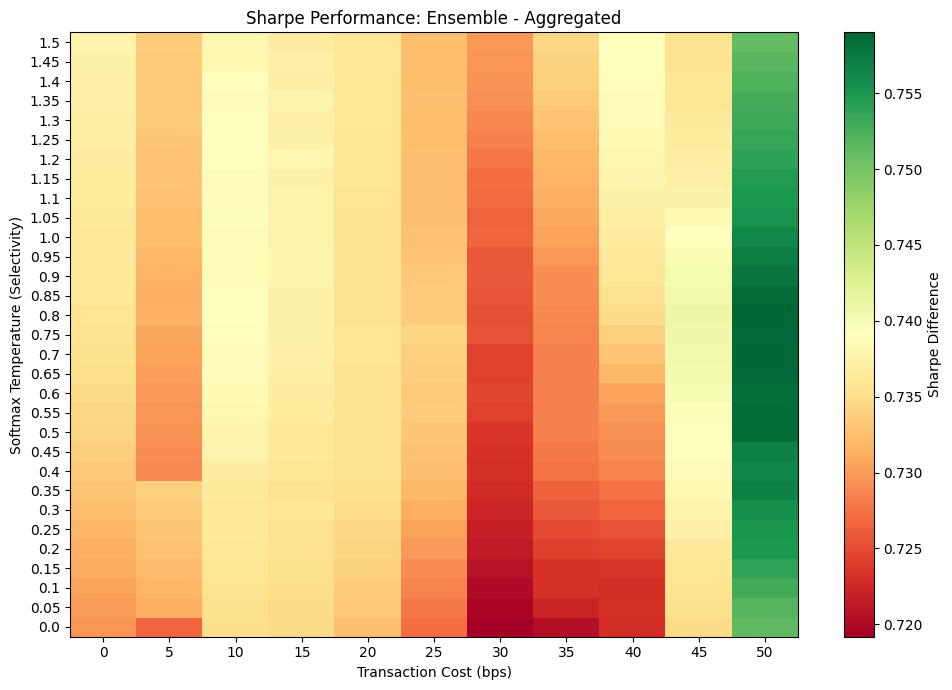
\includegraphics[width=0.58\textwidth]{Sharpe_ENS_Agg_N}
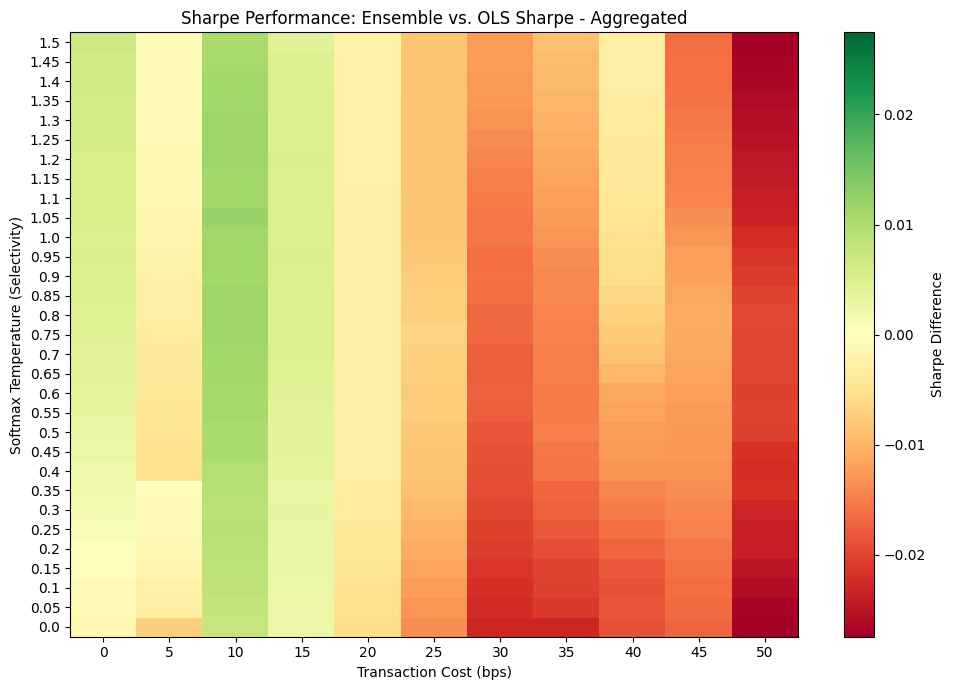
\includegraphics[width=0.55\textwidth]{Sharpe_ENS_OLS_Agg_N}
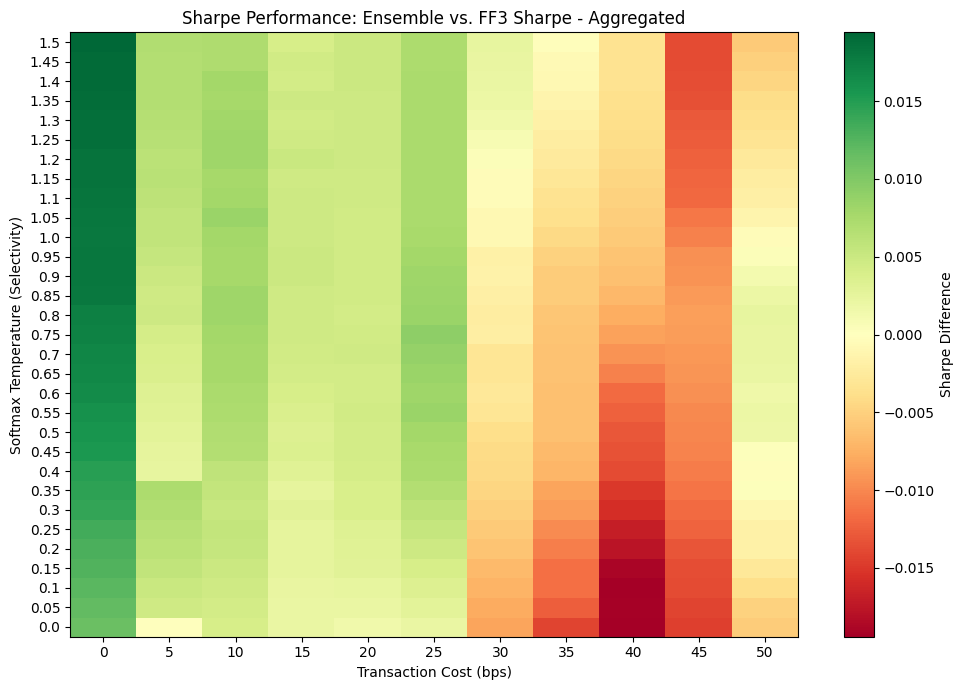
\includegraphics[width=0.55\textwidth]{Sharpe_ENS_FF3_Agg_N}
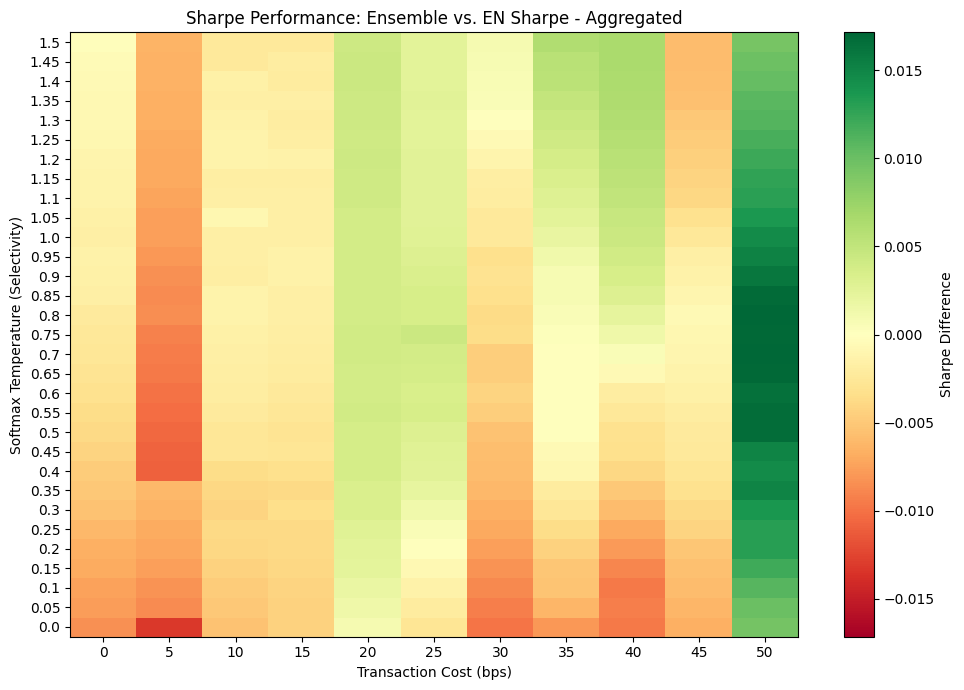
\includegraphics[width=0.55\textwidth]{Sharpe_ENS_EN_Agg_N}
\end{figure}

\vspace{5mm}

The ensemble factor investing strategy performs competitively with the three base models when measured by its Sharpe ratio, outperforming OLS and 3-factor FF models under low transaction cost regimes on average over the three datasets. The comparison to the Elastic Net base model was more varied, with weaker relative performance by the ensemble model under low transaction cost regimes in this instance but stronger relative performance at the 50 bps transaction cost level.\\

\break

\textbf{Aggregated Performance and Comparison to Base Models- Turnover:}\\

\begin{figure}[h!]
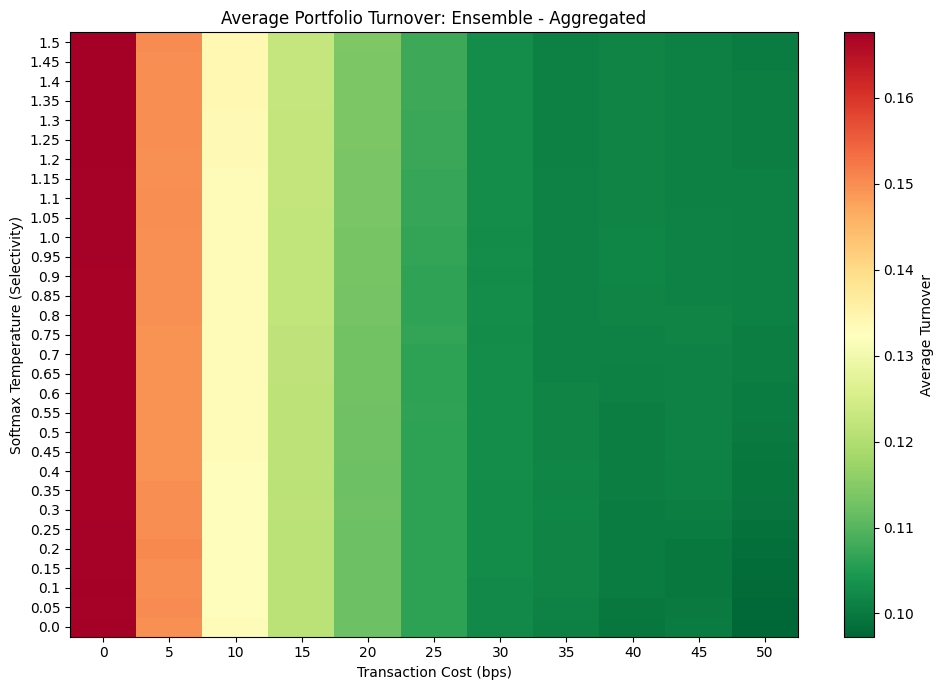
\includegraphics[width=0.58\textwidth]{Turn_ENS_Agg_N}
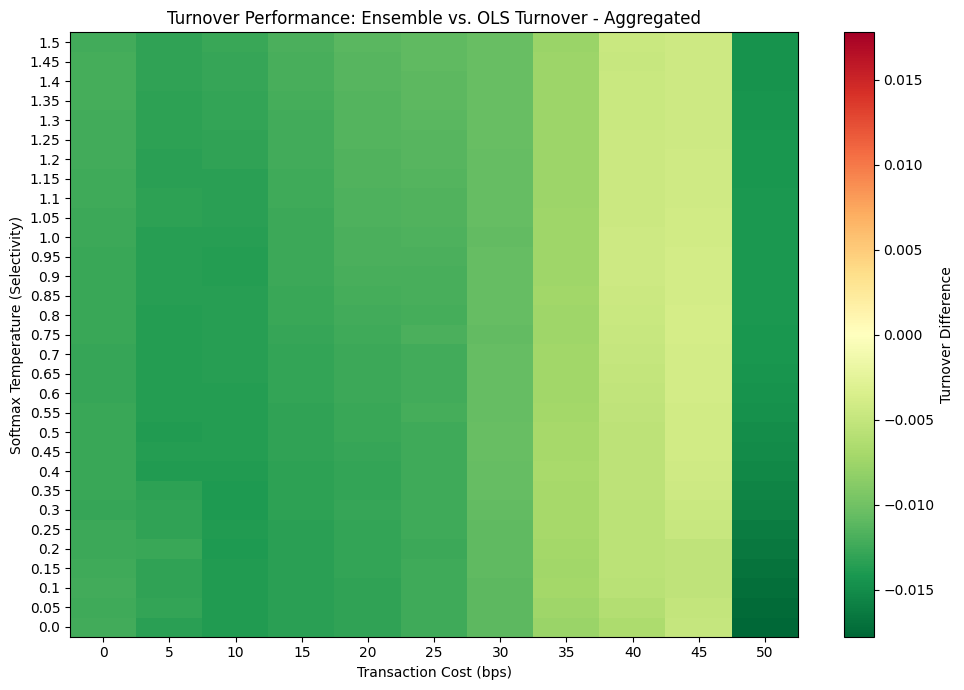
\includegraphics[width=0.55\textwidth]{Turn_ENS_OLS_Agg_N}
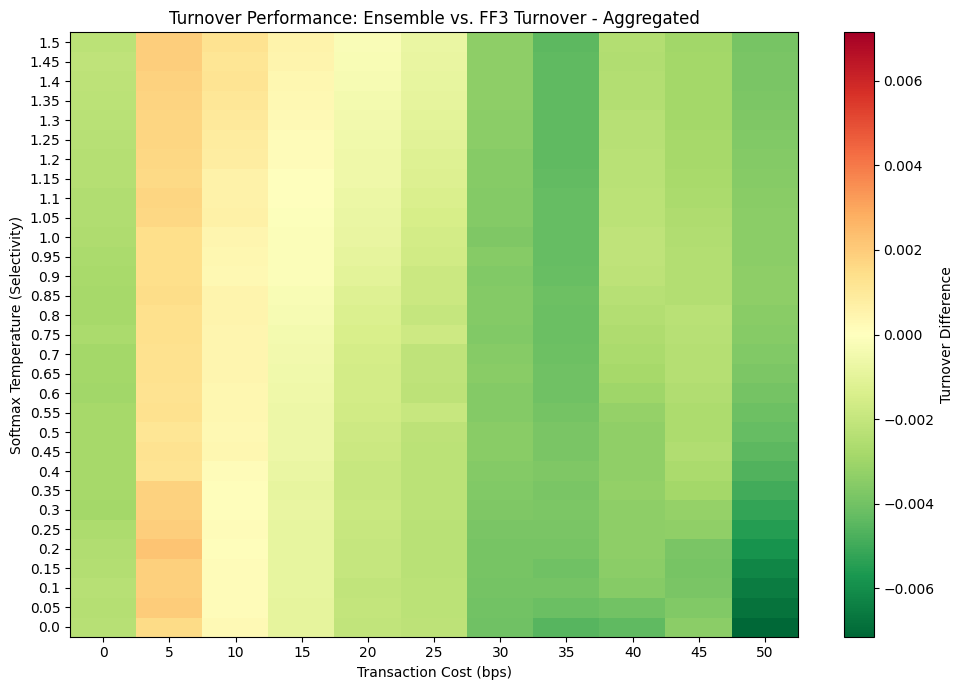
\includegraphics[width=0.55\textwidth]{Turn_ENS_FF3_Agg_N}
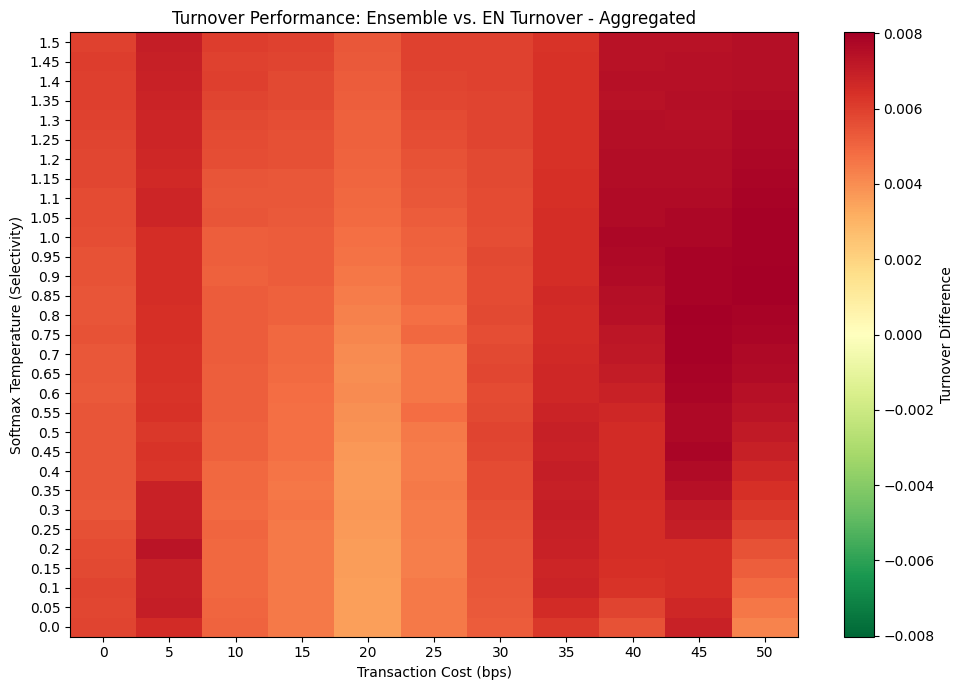
\includegraphics[width=0.55\textwidth]{Turn_ENS_EN_Agg_N}
\end{figure}

\vspace{5mm}

In absolute terms, the ensemble factor investing strategies of all temperature parameters see their average turnover reduced consistently as transaction costs increase (see top left). The ensemble factor investing strategy largely outperforms both OLS and FF3 in terms of average portfolio turnover but underperforms Elastic Net under all transaction cost, temperature parameter pairings.\\

\break

\textbf{Aggregated Temperature Comparison vs. Equal-Weighted Ensemble Method}\\

\begin{figure}[h!]
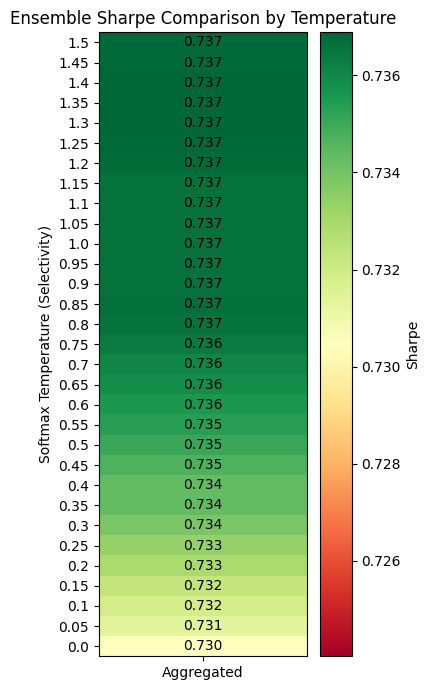
\includegraphics[width=0.5\textwidth]{Sharpe_ENS_Tempcomp_Agg}
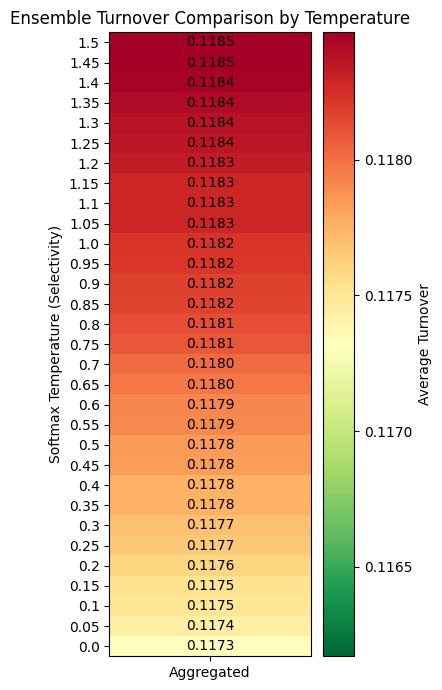
\includegraphics[width=0.514\textwidth]{Turn_ENS_Tempcomp_Agg}
\end{figure}

\break

\begin{figure}[h!]
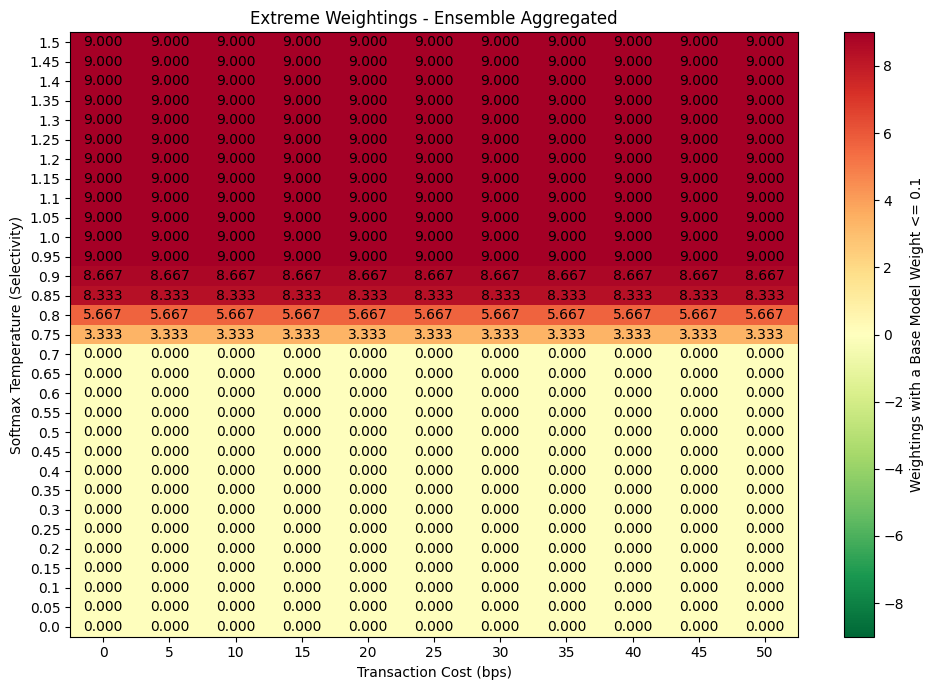
\includegraphics[width=0.90\textwidth]{Num_Ext_ENS_Agg}
\end{figure}

Transaction costs did not influence when the ensemble strategies produced extreme weightings (classified as at least one base model having a weighting of $\leq 0.1$. All strategies with temperature parameter 0.7 or less had no such weightings at any rebalance point. All strategies with temperature parameter 0.95 or higher produced extreme weightings at all rebalance points past the 18 month initial period (60-78 months in the each dataset) used to calibrate the base model weights.\\

\break

\section{Discussion of Results}

\textbf{On the potential benefit from ensembling}: \\

\emph{vs. OLS:}\\
SHARPE: Under low transaction costs, higher temperature (more extreme-weighting instances) ensemble strategies performed slightly better on average across the three datasets in terms of Sharpe ratio. \\
TURNOVER: Under low transaction costs, all ensemble strategies (across temperature range) outperformed OLS (by achieving lower turnover on average across the three datasets). This effect was less prominent in higher transaction cost regimes with the exception of 50 bps.\\
\emph{vs. FF3}:\\
SHARPE: Under low transacton costs, all ensemble strategies across the temperature parameter range outperformed FF3, with the most prominent difference appearing under 0 bps.\\
TURNOVER: The results were mixed under low transaction costs regimes, but under higher transaction cost regimes, all ensemble strategies outperformed FF3 on average over the three datasets.\\
\emph{vs. EN:}.\\
SHARPE: The results were mixed on average over the three datasets except for the 50 bps transaction cost regime, in which the medium-temperature ensemble strategies outperformed EN on average significantly, and the 5 bps transaction cost regime, in which the EN base model performed better on average across the three datasets.\\
TURNOVER: The EN strategy broadly outperformed the ensemble stategies across the temperature range in terms of average portfolio turnover.\\

\textbf{On the potential benefit from dynamically-updating weights vs. Equal-Weighted Ensemble}:\\
SHARPE: Slight benefit on average. Across the three datasets, the Sharpe ratio increased by about 1 percent on average across all transaction cost regimes at the 0.8-level temperature and above compared to the 0-level temperature (the equal-weighted ensemble).\\

TURNOVER: Slight detriment on average. Across the three datasets, the average turnover also increased by about 1 percent on average. It is worth noting that the average turnover metric is incorporated into the Sharpe ratio in the form of transaction costs depedent on level of turnover (which affect returns).\\


\textbf{Benefit from Transaction Costs}:\\

The addition of transaction costs had the effect of reducing overall portfolio turnover effectively in the ensemble strategies (across all temperature levels). The effect on the Sharpe ratio of the ensemble strategies was less consistent and was also temperature-level-dependent, but all average Sharpe ratios across all transaction costs and temperature levels stayed in the range of 0.72 to 0.76.\\

\break

\section{Limitations}

There are several key limitations to the performance and results of this project.\\

1. \textbf{Assuming flat transaction cost rates}:\\

For simplicity, there is no consideration of market impact from executing trades nor considerations about the liquidity of the 10 stocks in our universe (other than assuming the stocks are liquid enough to trade on demand every rebalancing period at the quantity of choice.\\

2. \textbf{Assuming no cash position and not considering risk measures}.\\

There is no value-at-risk, expected shortfall, or other risk calculation performed. In reality, some cash portion would likely need to be reserved.\\

3. \textbf{Using a 36-month evaluation window to calculate the factor mean.}\\

Due to the structure of the backtest, a shorter window had to be chosen. 36 months was judged to be significantly different from the 60 month factor return mean to yield meaningfully different asset allocations and long enough (2x the base model reweighting calibration window) to still yield a reasonable estimate of the future mean return vector.\\

4. \textbf{Limited difference between base models and ensemble models of varying temperature (base model selectivity)}\\

It is worth noting that the ensemble strategies (indexed by temperature range) only differ from each other after the first 18 months (at which there are enough mean return vector predictions and past realizations (3 x 6 months) to calibrate the softmax base model weightings for the ensemble step, so there is only a 54-month period of those strategies differing to measure differences in performance metrics like Sharpe ratio and turnover ratio. It is possible that a longer window to measure differences in the strategy may give different results.\\

5. \textbf{Universe of Stocks}\\

- A major limitation of this project is the selection bias inherent in the stock selection process. For the project backtests to be run as intended with the requisite data, it was necessary to find major public US equities that have 33 years of stock price history. However, it is worth noting that the focus of the project is to explore the potential benefits 1) of ensembling vs. using the base models and 2) of dynamically updating the base weights each rebalance period vs. using the equal-weighted ensemble method.\\

\break

\section{References}

Shao, J. (V), Miao, X. (A), Zhang, Y. (J), Li, X. (S) (2025). MMF 1921. Operations Research, Project 2. \\

J. (V) Shao, personal communication, June - August (2026).\\

Zou, H., Hastie, T. (2003). Stanford University, USA. Regularization and variable selection via the elastic net.\\

Li, F., Chow, T-M., Pickard, A., Garg, Y. (2019) Financial Analysts Journal. Transaction Costs of Factor-Investing Strategies.\\

\break

\section{Version History}

\vspace{5mm}

\textbf{Version 1: July 22, 2026}\\

- Ran initial backtests and displayed results in table format.\\

- The factor returns were not standardized when used for elastic net method.\\

- 6 month calibration window was used for the base model weights, resulting in noise-chasing. \\

- The other issue with updating the base model weights was that the errors used were not standardized in the initial build. The updated version standardized the weighted (exponentially using parameter $\lambda_W = 0.75$) root mean squared error between the predicted mean excess asset return vector of each base model and the actual sample mean vector over each of the three 6-month periods.\\

- Covariance matrix base model weights were also updated using this 6 month calibration window. The updated design was used after discussions with Shao, V. with the goal of accentuating differences in the mean return vector estimates (to allow for the base model reweighting methodology to be tested) while preserving a robust equal-weighted covariance matrix to use as the ensemble estimate.\\

- The elastic net $\lambda_1, \lambda_2$ tuning was inside of the backtest/rebalancing loop. This created a massive redundancy when the previous backtest was run. The $\lambda_1, \lambda_2$ tuning was the most expensive part of the backtest computationally already. The redundancy stemmed from the fact that the chosen $\lambda_1, \lambda_2$ are independent of the (transaction cost, temperature) parameter pair. In the initial design, there were only 6 (transaction cost, temperature) pairs

- It was later discovered that the base model mean vectors were identical under this setup (which led to the 36-month) window being used for the mean return vector calculation rather than the standard 60-month rolling window of data used previously. This was masked in the initial setup due to the differing covariance matrices\\

\emph{Discussion: Base model mean vectors identical under previous design.} \\

Under the previous implementation, the expected return vector for each base model was estimated as
\[ \hat{\mu}_i = \hat{\alpha}_i +\hat{B}_i^{\top}\bar{F} \],\\

where $\bar{F}$ was the sample mean of the factor returns over the same 60-month window used to estimate the factor loadings.

For the OLS-based models, the inclusion of an intercept implies that the fitted regression passes through the sample means:
\[\bar{y}_i=\hat{\alpha}_i +\hat{B}_i^{\top}\bar{F}\] .\\
Consequently,
$\hat{\mu}_i=\bar{y}_i$,
regardless of the estimated factor loadings, where we note that $\bar{y}_i$ depends only on the time $T$, not the factor exposures. Thus, despite OLS and FF3 producing different factor exposures, their estimated mean return vectors were identical when the same observations were used both for model estimation and for calculating $\bar{F}$.

As a result, changing the temperature parameters (and thus the softmax weights) assigned to these base models had no effect on the ensemble mean vector. \\

A similar effect occurred for the Elastic Net model. The factor returns were standardized over the estimation window and the intercept was left unpenalized. Consequently, the intercept adjusts to the sample mean of each asset's returns, while the standardized factors have zero sample mean. Evaluating the fitted model at the factor means from that same estimation window therefore also produces $\hat{\mu}_{\text{EN}} \approx \bar{y}$. Thus, all three base models produced identical mean return vectors despite having different factor-loading estimates.\\

The revised methodology avoids this mechanical equality by calculating the factor mean over a 36-month window rather than the full 60-month model-estimation window.\\

\emph{A Note on the Identical Mean Vectors:} This was discovered when it was seen that the performance metrics were largely identical across the temperature parameter range because a common covariance matrix was implemented. When the mean vectors were inspected at each rebalancing step, they were identical to eight decimal places for all 10 assets. Under the previous setup (Draft 3), it was invisible without inspecting the mean return vectors at each rebalancing step, which was never done.\\

My understanding is that this may occur in any OLS-based regression (ie. BSS and 3-factor/5-factor FF methods) as well as any norm-penalizing setup (LASSO, Ridge, and Elastic Net) in which the intercept term is not penalized (as seen from the fact that the EN vectors were also identical.\\

Following the adjustment of the mean factor return to be over the previous 36 rather than 60 months, the mean return vectors using each base model regression were inspected again and material differences appeared. The covariance matrix estimation still uses $T=60$ factor return points (in the code there is an $\bar{F}_{60}$ used in the covariance calculation and a $\bar{F}_{36}$ used in the mean vector calculation).\\

\emph{Proof that the mean vectors were indeed identical:}\\

General Optimization which covers OLS, FF3, FF5, BSS, LASSO, Ridge, EN:\\

The general minimization is:\\

\[ \min_{\alpha_i, \beta_i} [ \sum_{t=1}^T \epsilon_i^2 + \lambda_1 \|\beta_i\|_1 + \lambda_2 \|\beta_i\|_2^2 ] \hspace{15mm} (1) \] \\

\[ = \min_{\alpha_i, \beta_i} [ \sum_{t=1}^T (y_i^{(t)} - \alpha_i - \beta_i^{\top} F^{(t)})^2 + \lambda_1 \|\beta_{i}\|_1 + \lambda_2 \|\beta_{i}\|_2^2 ] \hspace{6mm} =:\min_{\alpha_i, \beta_i} (L) \] where we note $\alpha_i$ is not penalized and that $\lambda_1 = \lambda_2 = 0$ for OLS, FF3, FF5, BSS.\\

\[ \Rightarrow \frac{\partial L }{\partial \alpha_i } = -2 \sum_{t=1}^T (y_i^{(t)} - \alpha_i - \beta_i^{\top} F^{(t)}) \] \\

Setting $\frac{\partial L}{\partial \alpha_i} = 0$ and solving for optimal $\hat{\alpha_i}$, \\

\[ \Rightarrow \hat{\alpha_i} = \frac{1}{T} \sum_{t=1}^{T} y_i^{(t)} - \frac{1}{T} \sum_{t=1}^T \hat{\beta}_i^{\top} F^{(t)} = \bar{y_i} - \hat{\beta}_i^{\top} \bar{F} \] \\

\[ \Rightarrow \hat{\mu}_i = \hat{\alpha}_i + \hat{\beta_i}^{\top} \bar{F} (\text{per mean asset return vector estimate methodology}) = (\bar{y_i} - \hat{\beta}_i^{\top} \bar{F}) +  \hat{\beta_i}^{\top} \bar{F} = \bar{y_i} \hspace{3mm} \forall i \in \{1,...,n\} \] \\

\[ \Rightarrow \hat{\mu} = \bar{y} \] for all base models with general optimization setup (1). We note that this only holds when the same $T$ is used to calculate $\bar{F}$ in the mean asset return vector estimate and $\bar{F}$ in the $\hat{\alpha}, \hat{\beta}$ calculation. The new methodology uses $\bar{F}_{36}$ in the mean asset return vector estimate which differs (in all practical cases) from $\bar{F}_{60}$ used in the $\hat{\alpha}, \hat{\beta}$ calculation for each of the base models.\\

\vspace{5mm}

\break

\section{Appendix}

\textbf{Sharpe Ratio Aggregation and Base Model Comparison with Values}\\

\vspace{5mm}

\begin{figure}[h!]
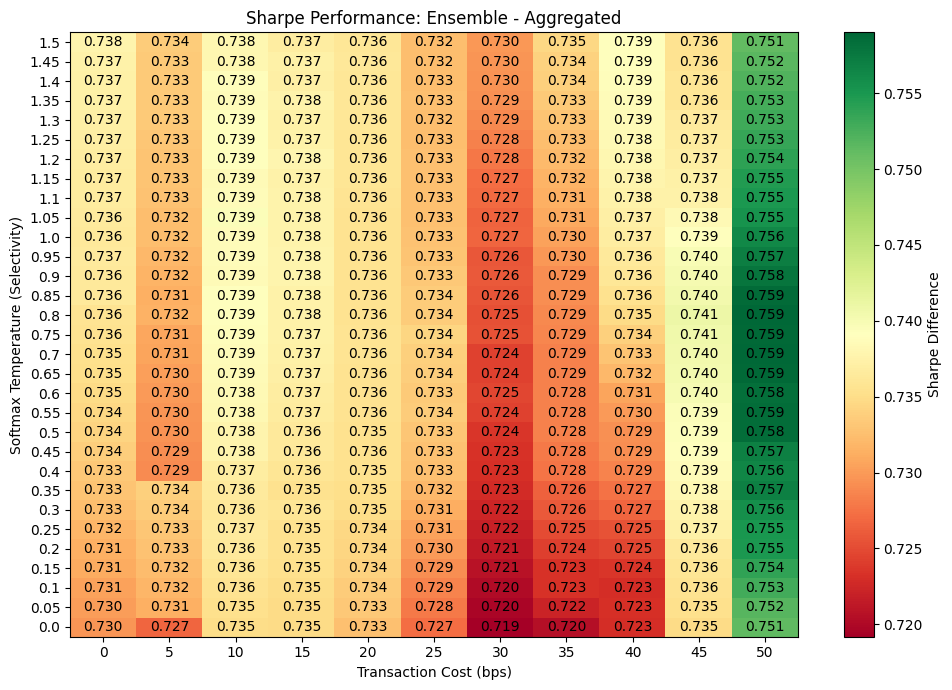
\includegraphics[width=0.75\textwidth]{Sharpe_ENS_Agg}
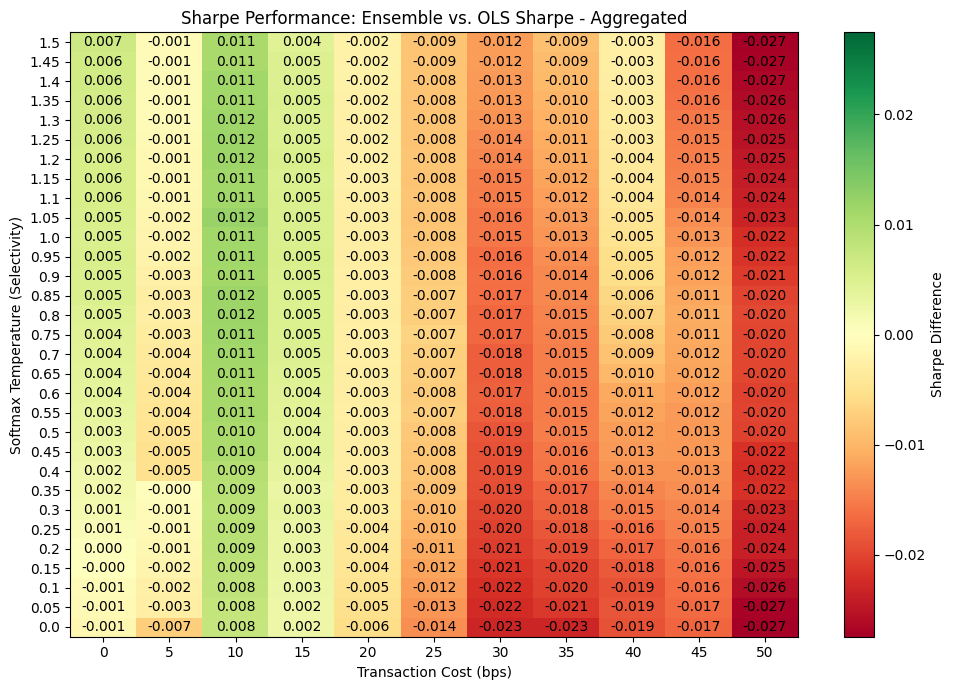
\includegraphics[width=0.75\textwidth]{Sharpe_ENS_OLS_Agg}
\end{figure}

\break

\begin{figure}[h!]
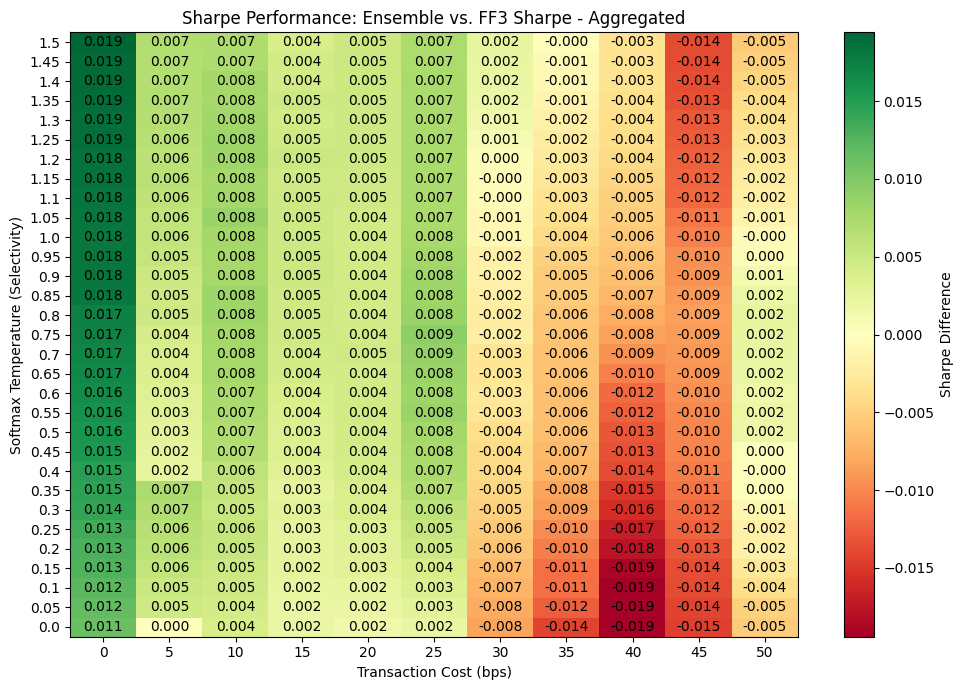
\includegraphics[width=0.75\textwidth]{Sharpe_ENS_FF3_Agg}
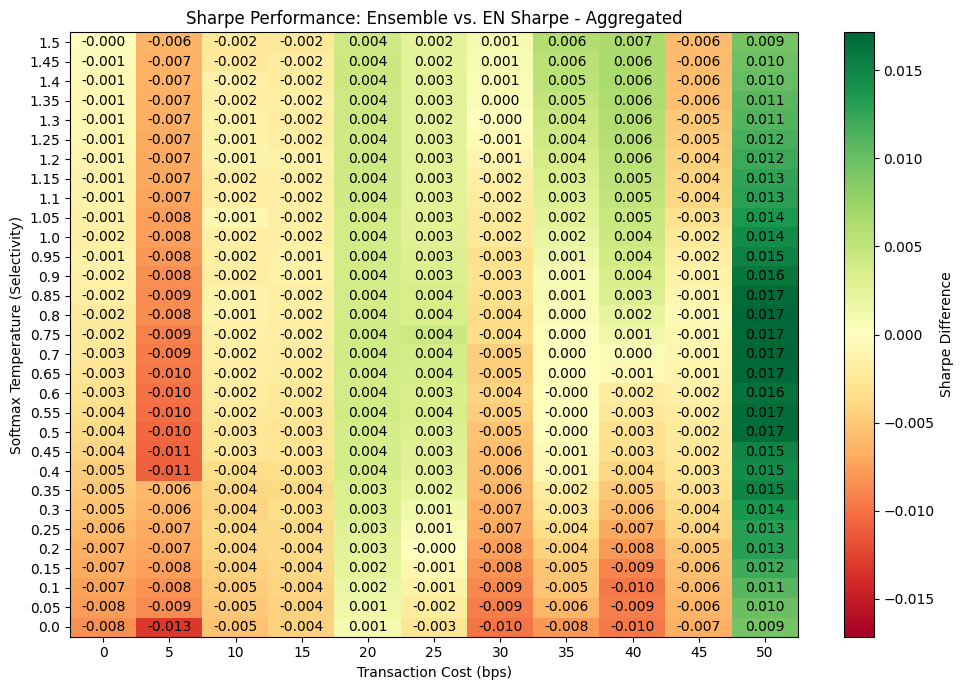
\includegraphics[width=0.75\textwidth]{Sharpe_ENS_EN_Agg}
\end{figure}

\break

\textbf{Turnover Aggregation and Base Model Comparison with Values}\\

\vspace{5mm}

\begin{figure}[h!]
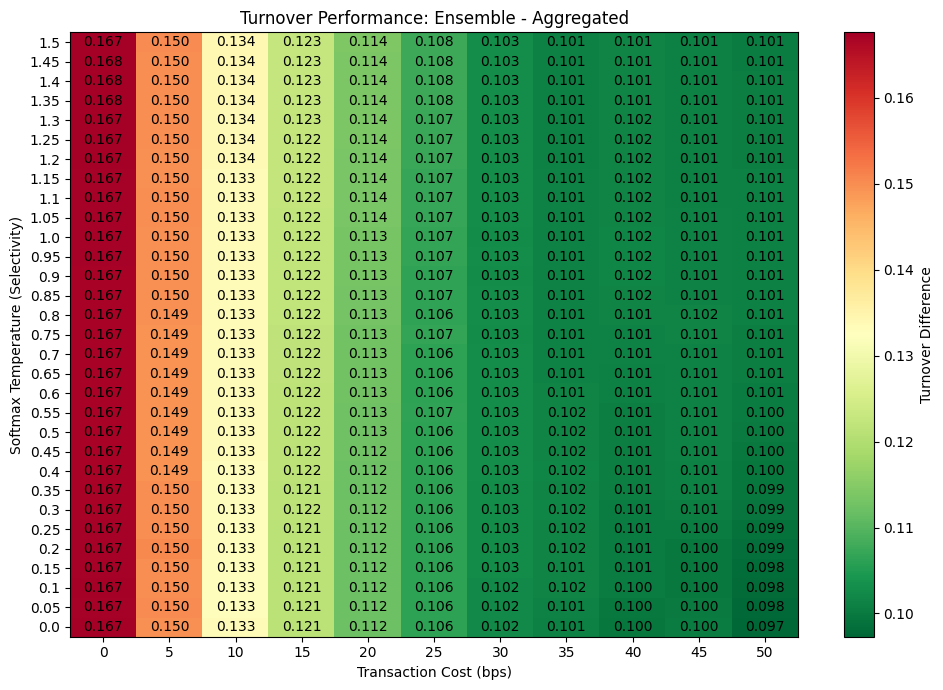
\includegraphics[width=0.75\textwidth]{Turn_ENS_Agg}
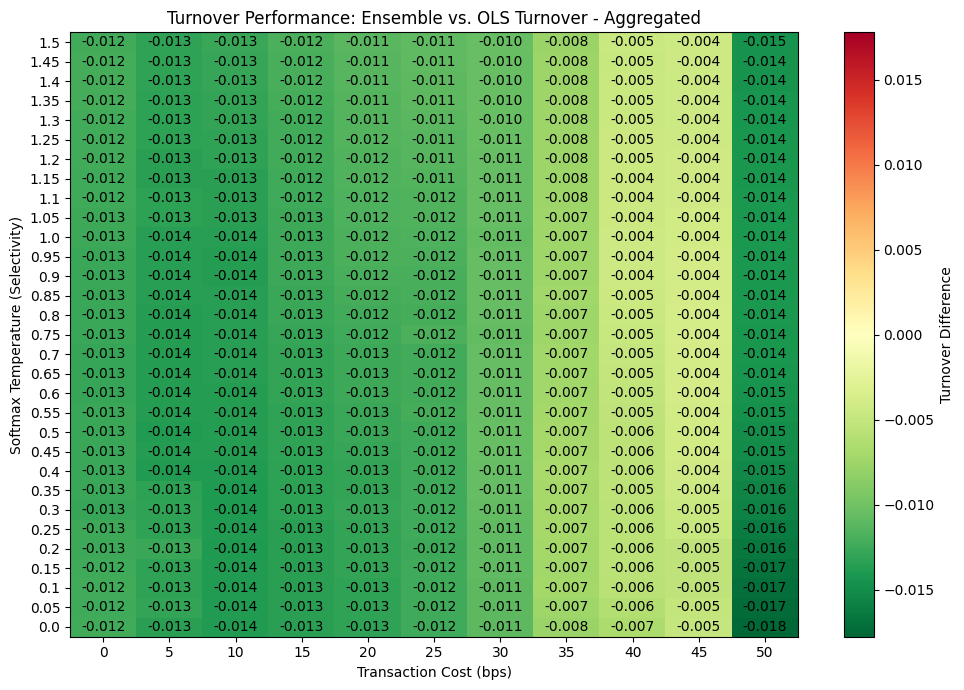
\includegraphics[width=0.75\textwidth]{Turn_ENS_OLS_Agg}
\end{figure}

\break

\begin{figure}[h!]
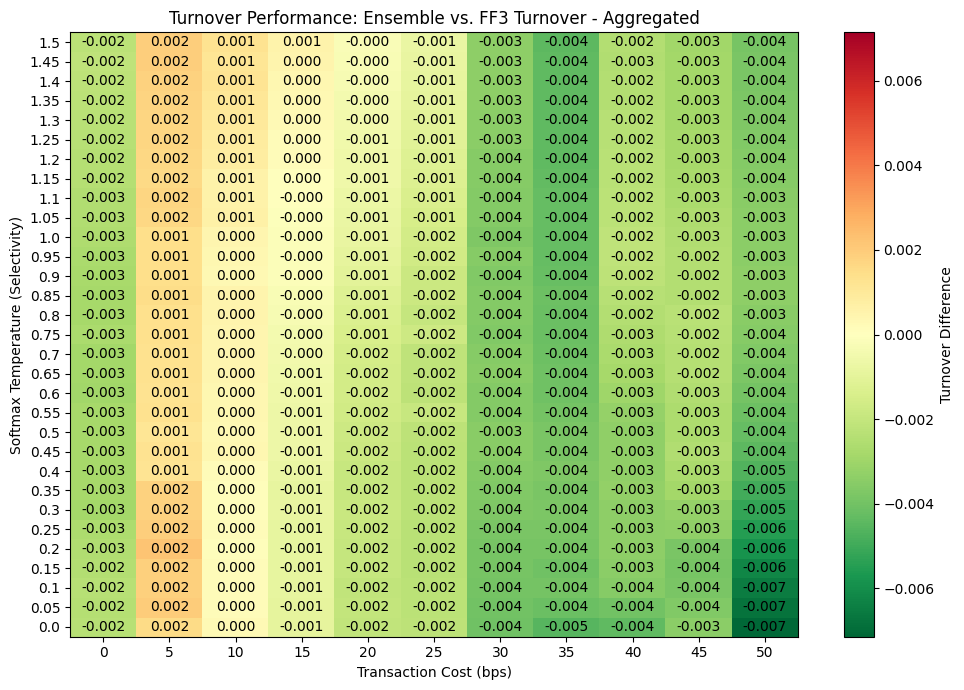
\includegraphics[width=0.75\textwidth]{Turn_ENS_FF3_Agg}
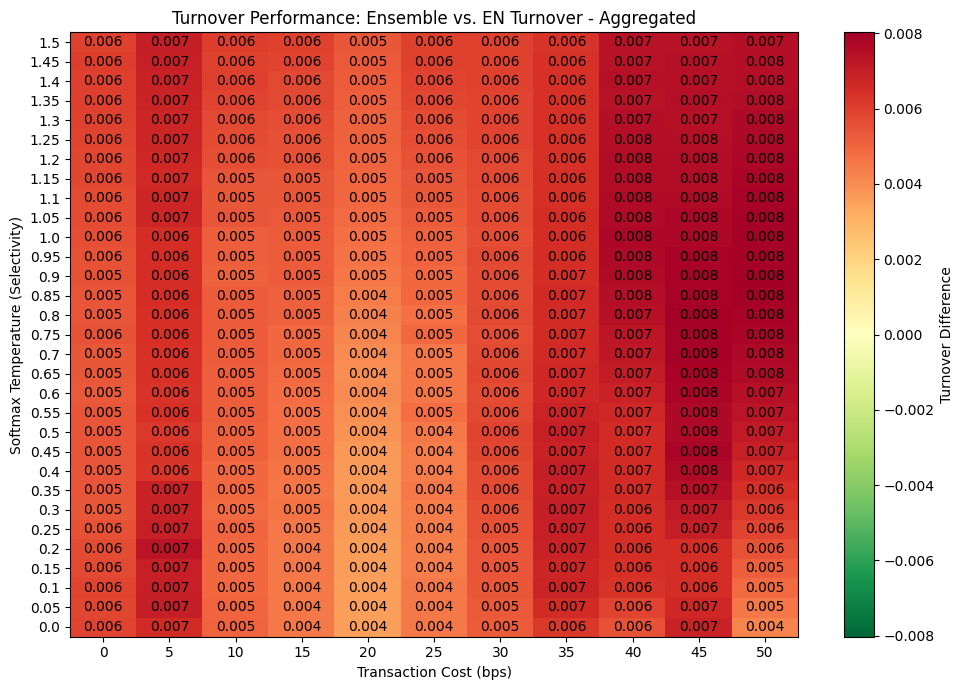
\includegraphics[width=0.75\textwidth]{Turn_ENS_EN_Agg}
\end{figure}

\break

\textbf{Sharpe Performance and Base Model Comparison with Values- Dataset 1}\\

\begin{figure}[h!]
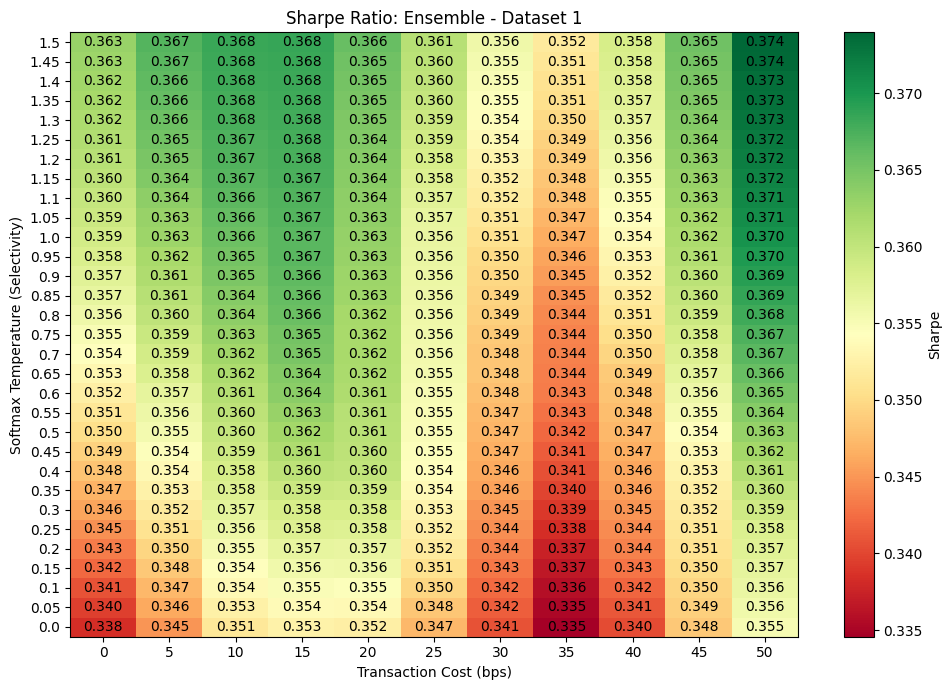
\includegraphics[width=0.75\textwidth]{Sharpe_ENS_D1}
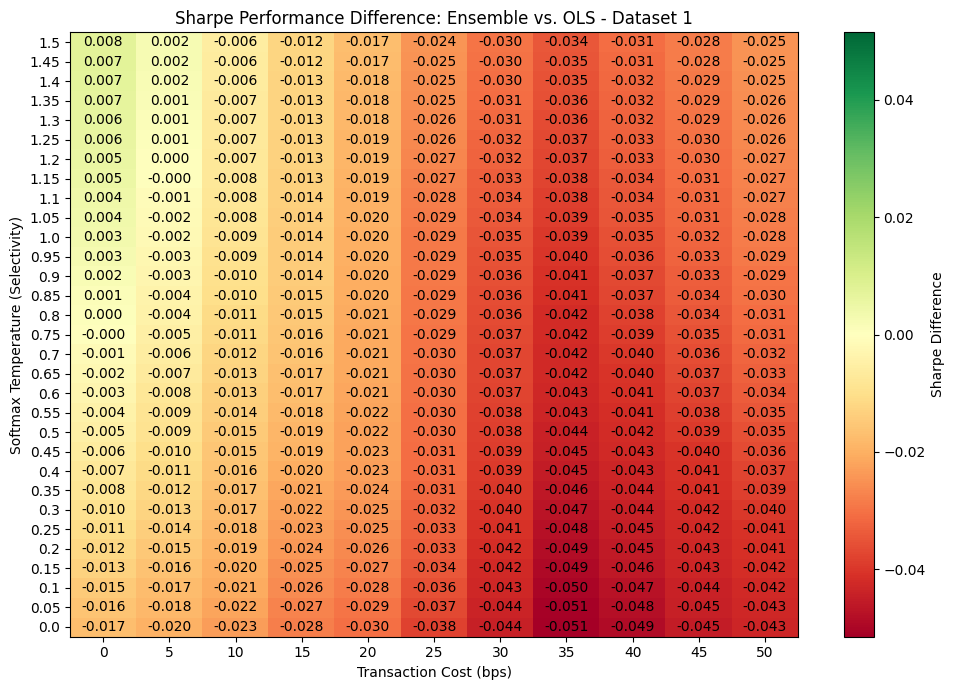
\includegraphics[width=0.75\textwidth]{Sharpe_ENS_OLS_D1}
\end{figure}

\break

\begin{figure}[h!]
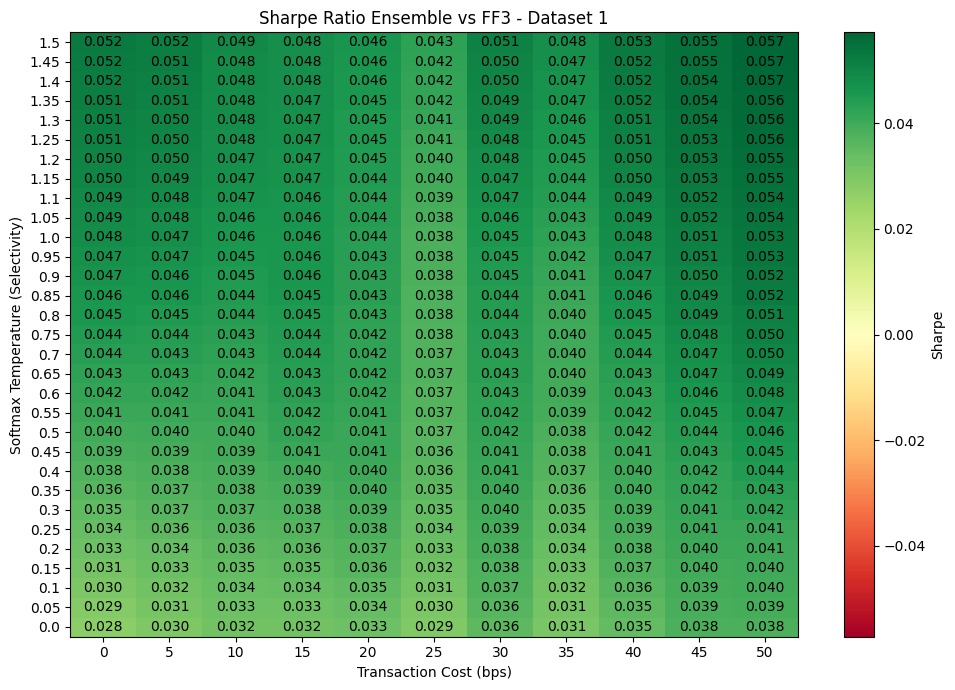
\includegraphics[width=0.75\textwidth]{Sharpe_ENS_FF3_D1}
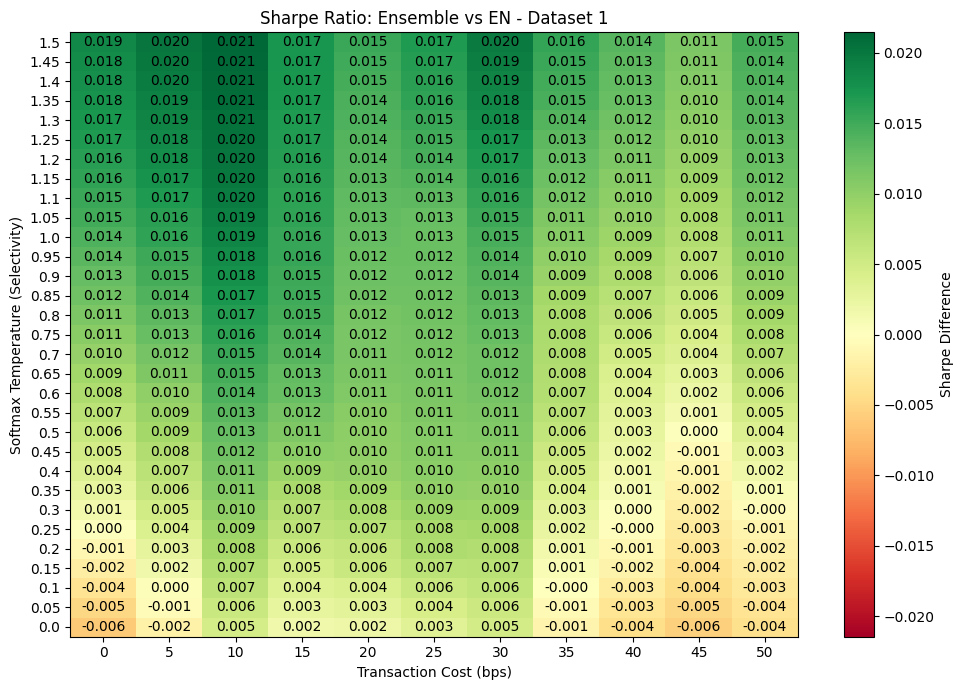
\includegraphics[width=0.75\textwidth]{Sharpe_ENS_EN_D1}
\end{figure}

\break

\textbf{Sharpe Performance and Base Model Comparison with Values- Dataset 2}\\

\begin{figure}[h!]
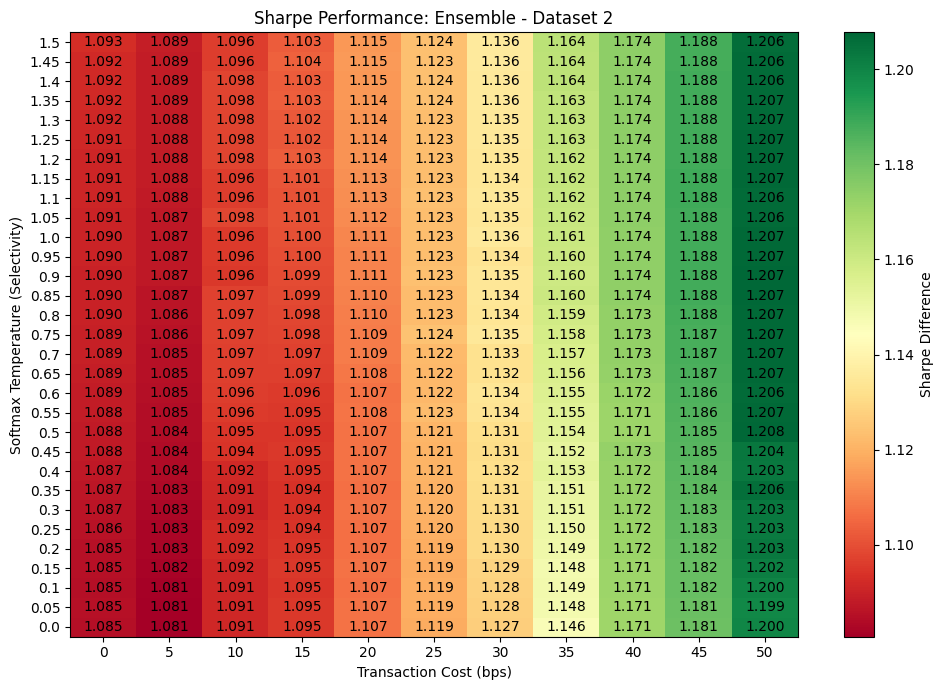
\includegraphics[width=0.75\textwidth]{Sharpe_ENS_D2}
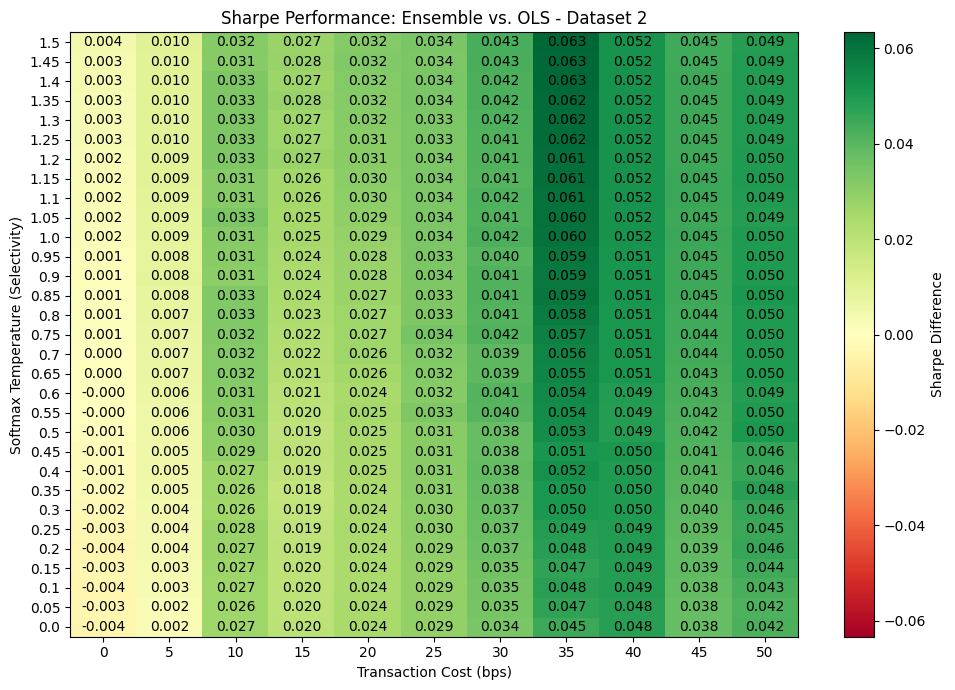
\includegraphics[width=0.75\textwidth]{Sharpe_ENS_OLS_D2}
\end{figure}

\break

\begin{figure}[h!]
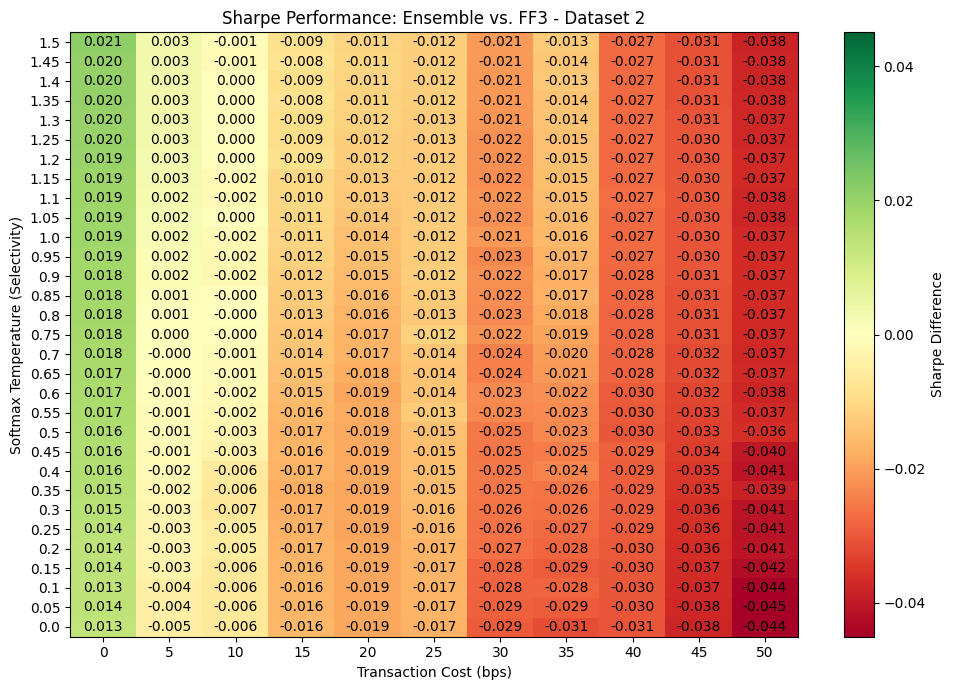
\includegraphics[width=0.75\textwidth]{Sharpe_ENS_FF3_D2}
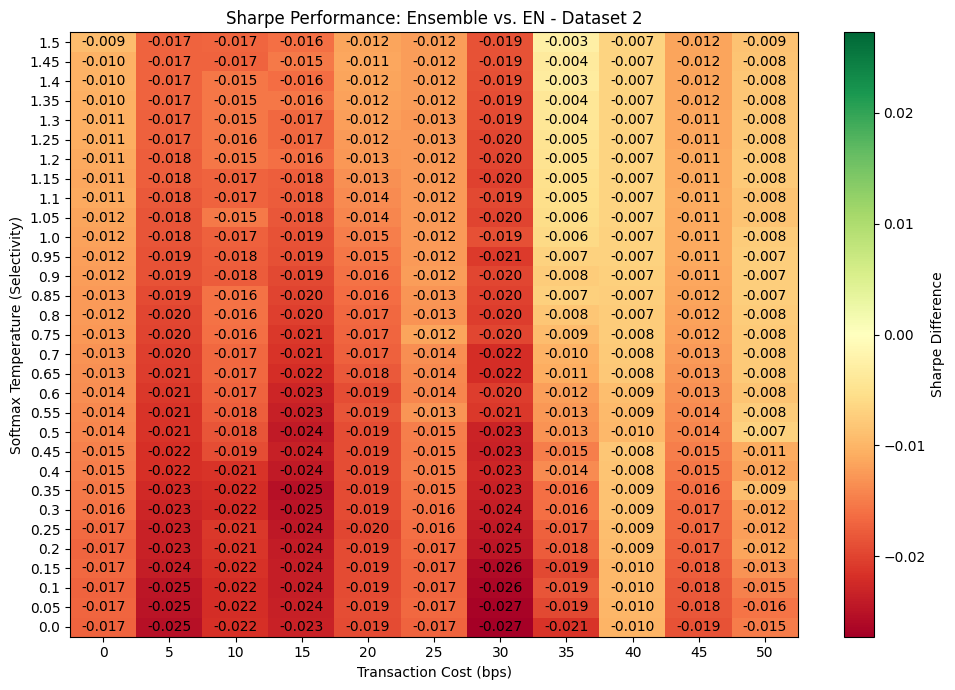
\includegraphics[width=0.75\textwidth]{Sharpe_ENS_EN_D2}
\end{figure}

\break

\textbf{Sharpe Performance and Base Model Comparison with Values- Dataset 3}\\

\begin{figure}[h!]
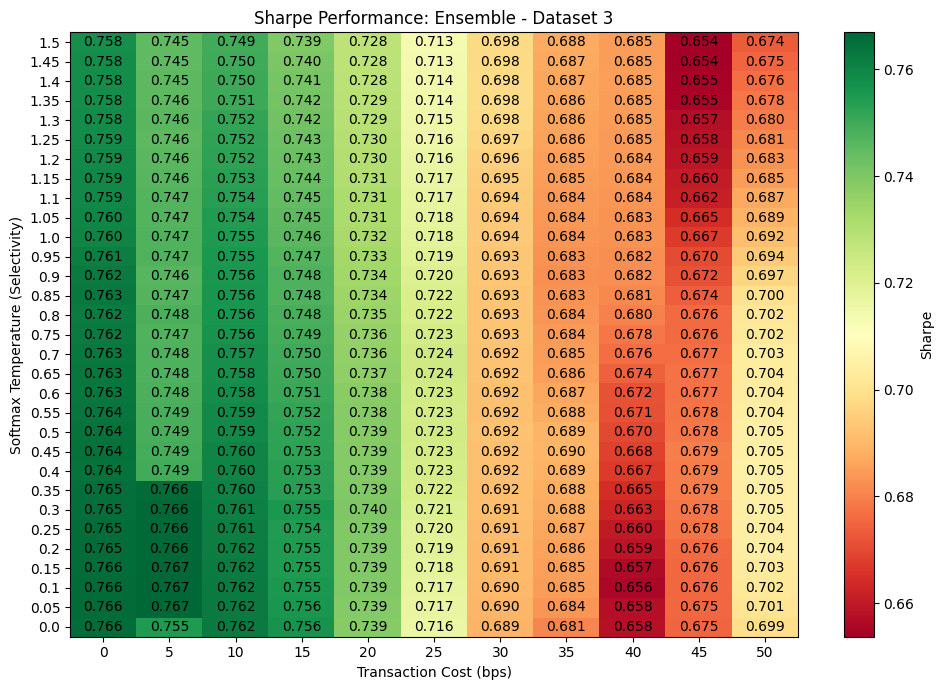
\includegraphics[width=0.75\textwidth]{Sharpe_ENS_D3}
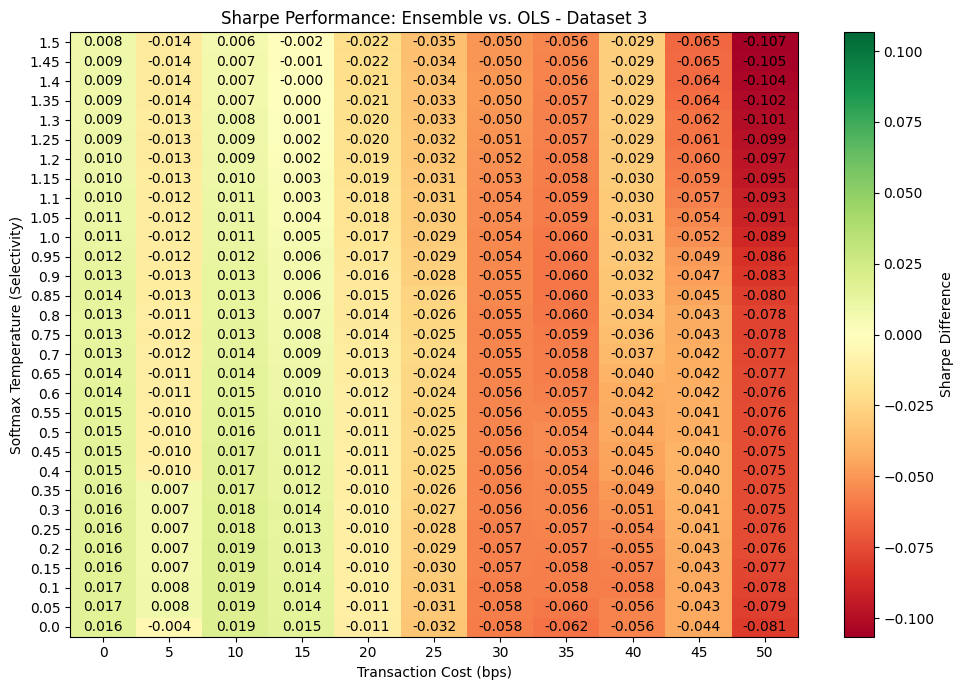
\includegraphics[width=0.75\textwidth]{Sharpe_ENS_OLS_D3}
\end{figure}

\break

\begin{figure}[h!]
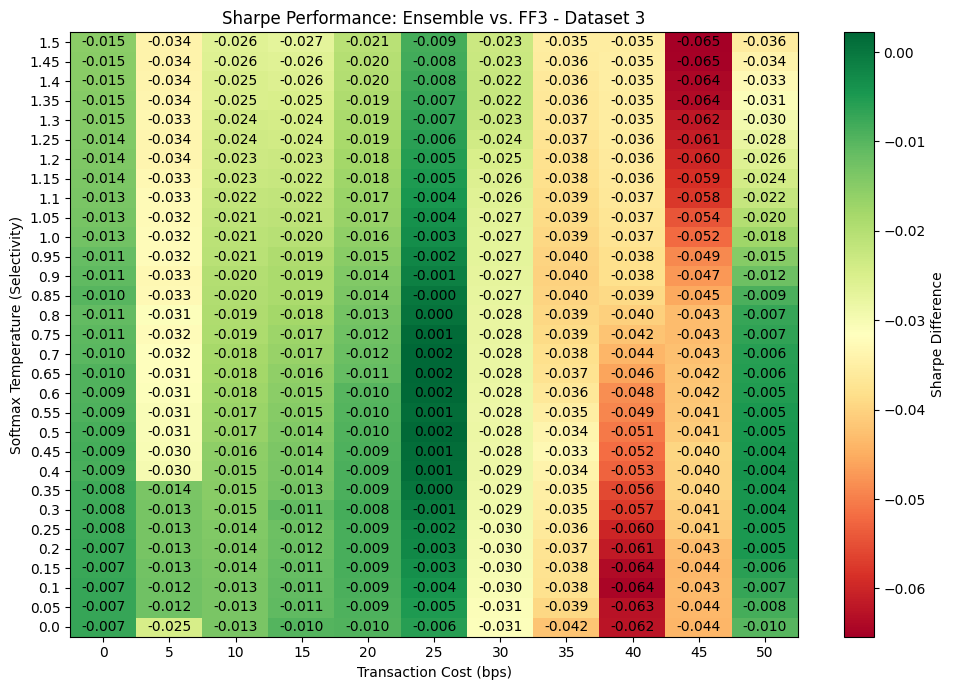
\includegraphics[width=0.75\textwidth]{Sharpe_ENS_FF3_D3}
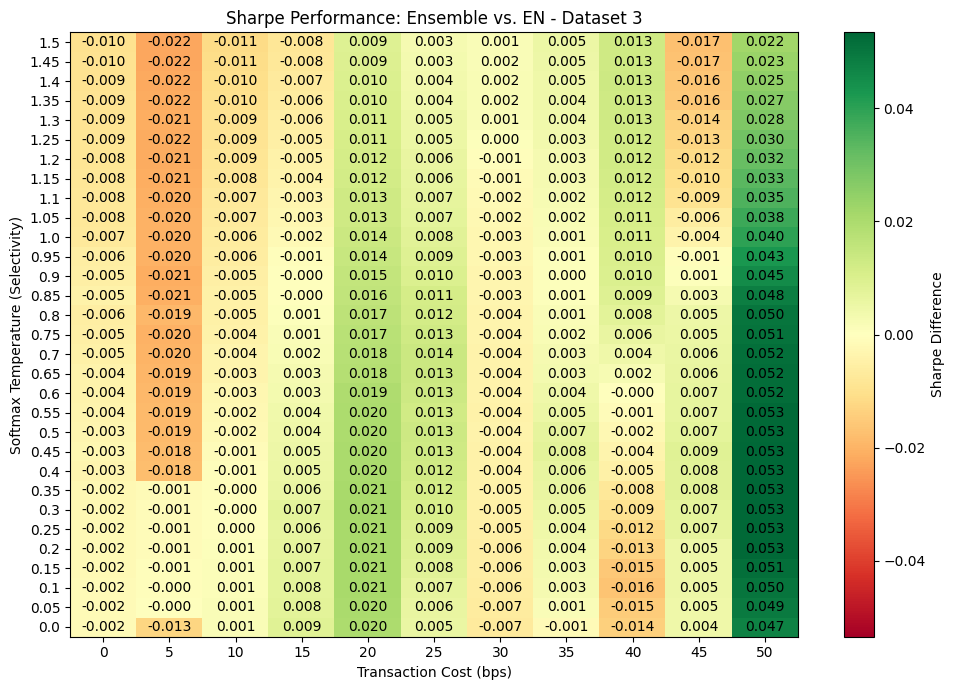
\includegraphics[width=0.75\textwidth]{Sharpe_ENS_EN_D3}
\end{figure}

\break

\textbf{Turnover Performance and Base Model Comparison with Values - Dataset 1}\\

\begin{figure}[h!]
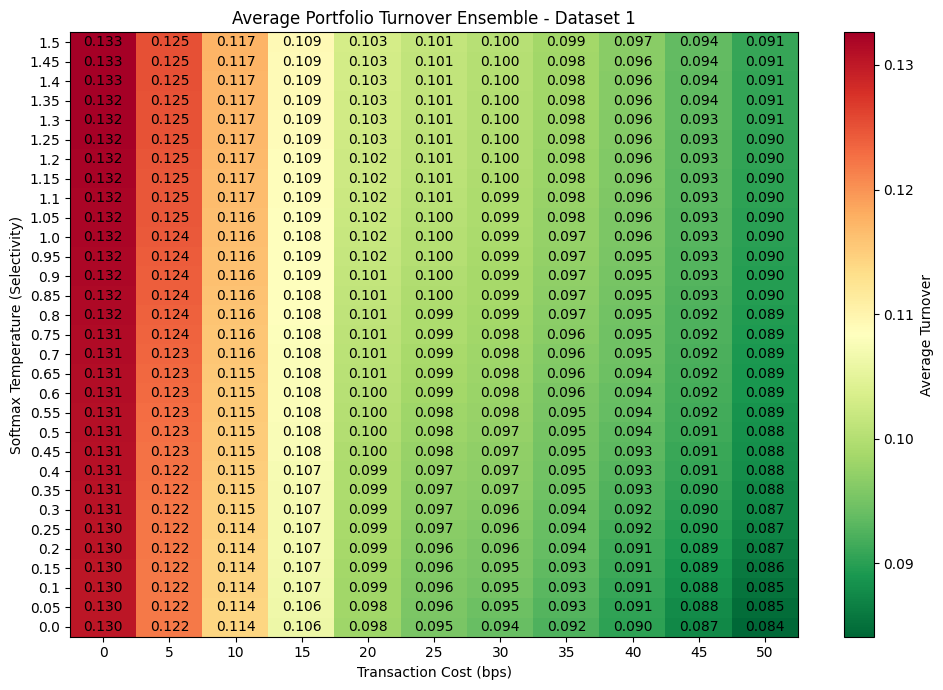
\includegraphics[width=0.75\textwidth]{Turn_ENS_D1}
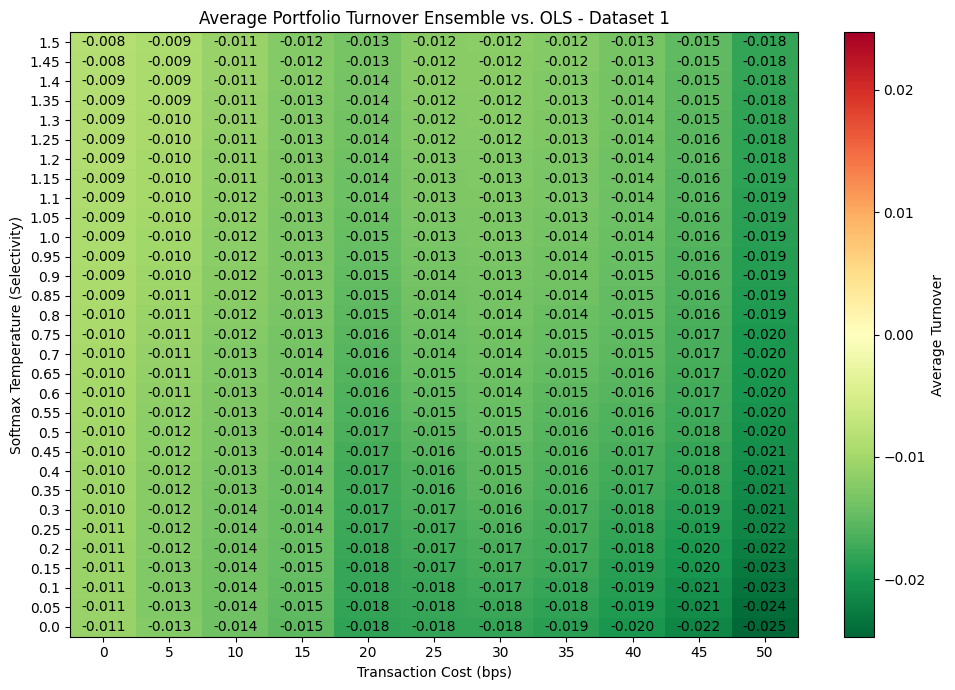
\includegraphics[width=0.75\textwidth]{Turn_ENS_OLS_D1}
\end{figure}

\break

\begin{figure}[h!]
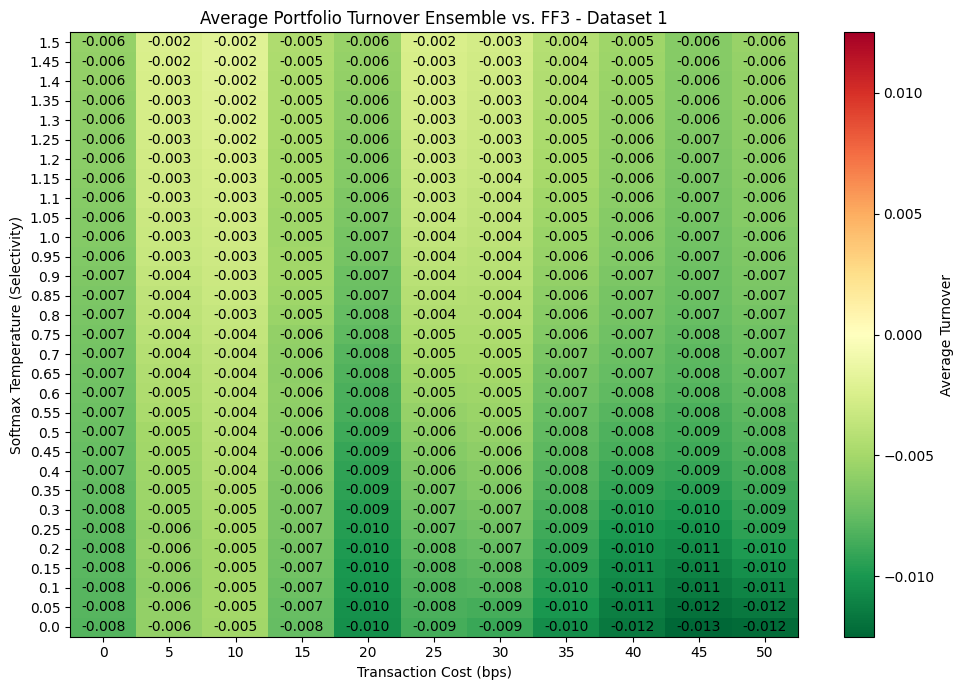
\includegraphics[width=0.75\textwidth]{Turn_ENS_FF3_D1}
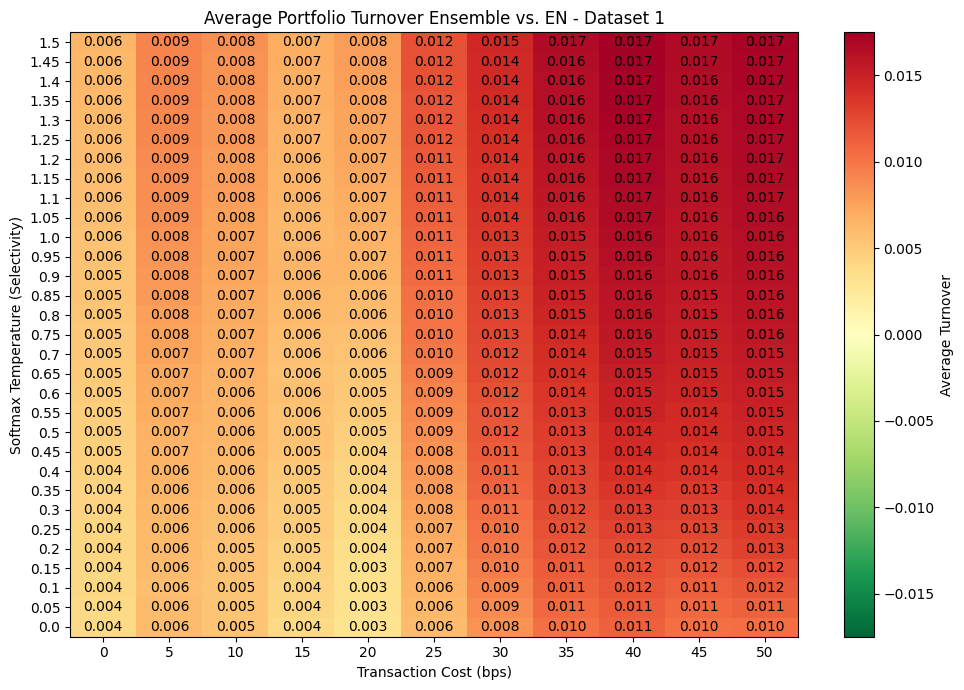
\includegraphics[width=0.75\textwidth]{Turn_ENS_EN_D1}
\end{figure}

\break

\textbf{Turnover Performance and Base Model Comparison with Values - Dataset 2}\\

\begin{figure}[h!]
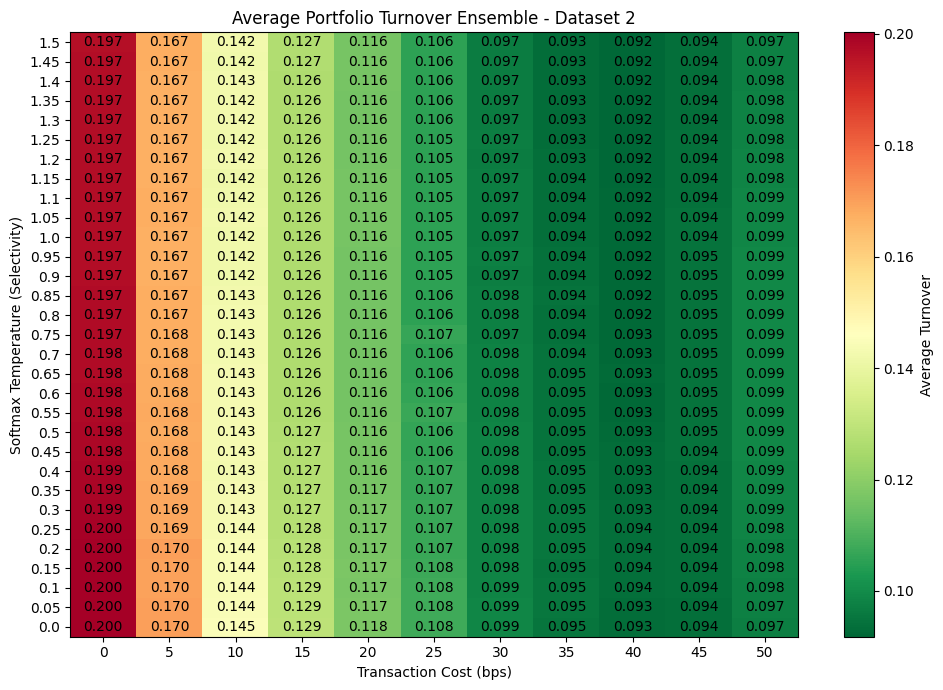
\includegraphics[width=0.75\textwidth]{Turn_ENS_D2}
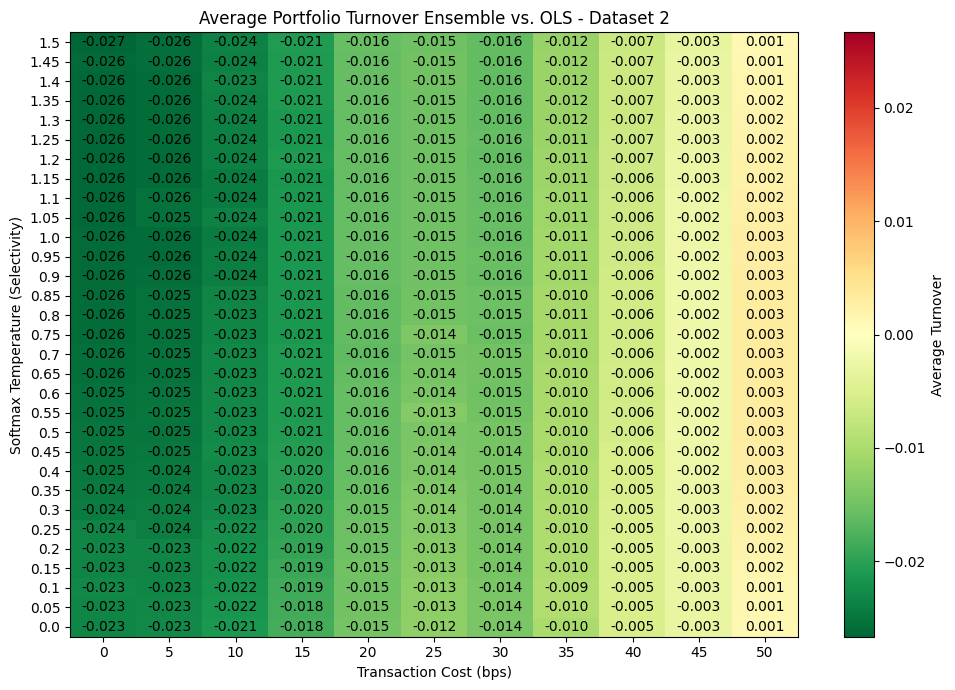
\includegraphics[width=0.75\textwidth]{Turn_ENS_OLS_D2}
\end{figure}

\break

\begin{figure}[h!]
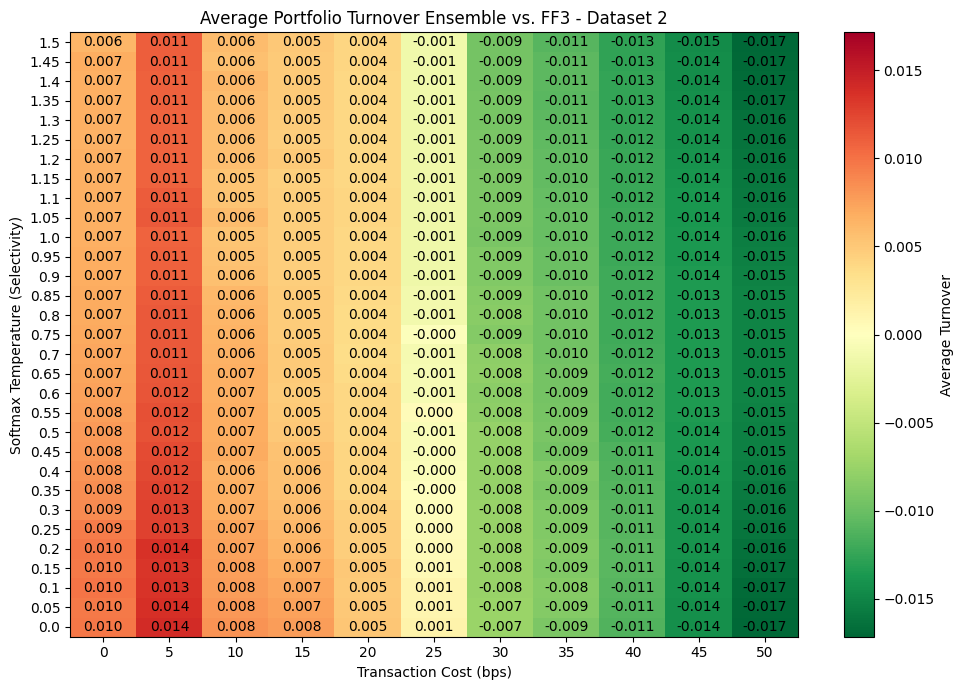
\includegraphics[width=0.75\textwidth]{Turn_ENS_FF3_D2}
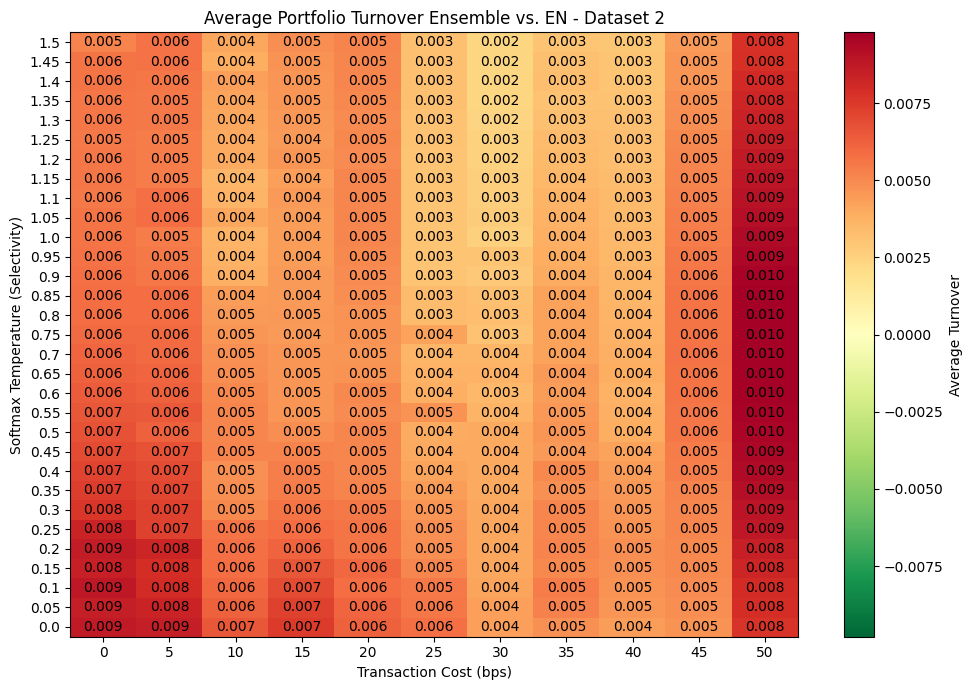
\includegraphics[width=0.75\textwidth]{Turn_ENS_EN_D2}
\end{figure}

\break

\textbf{Turnover Performance and Base Model Comparison with Values - Dataset 3}\\

\begin{figure}[h!]
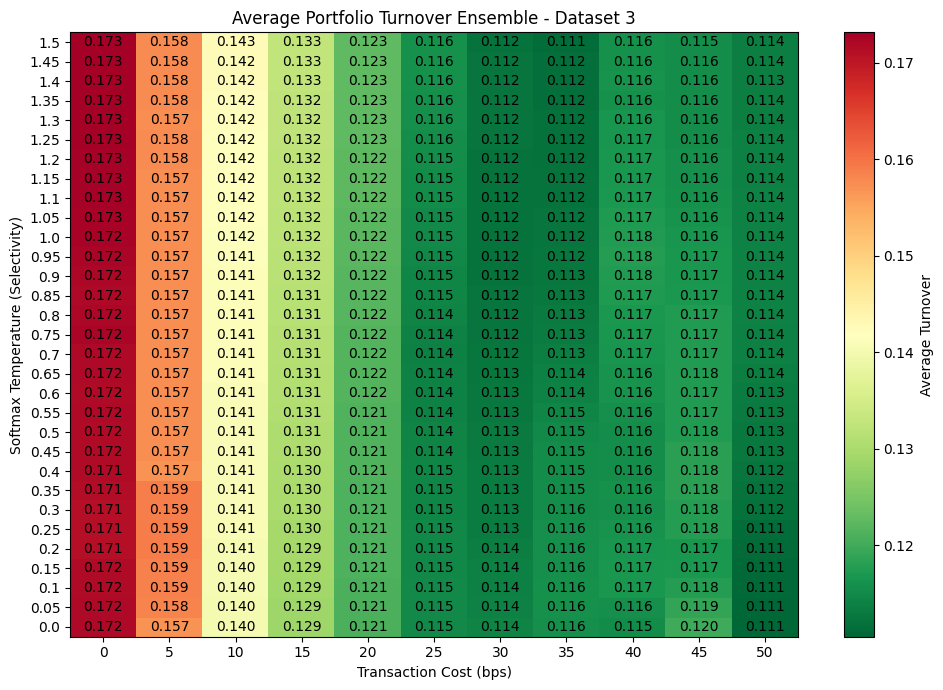
\includegraphics[width=0.75\textwidth]{Turn_ENS_D3}
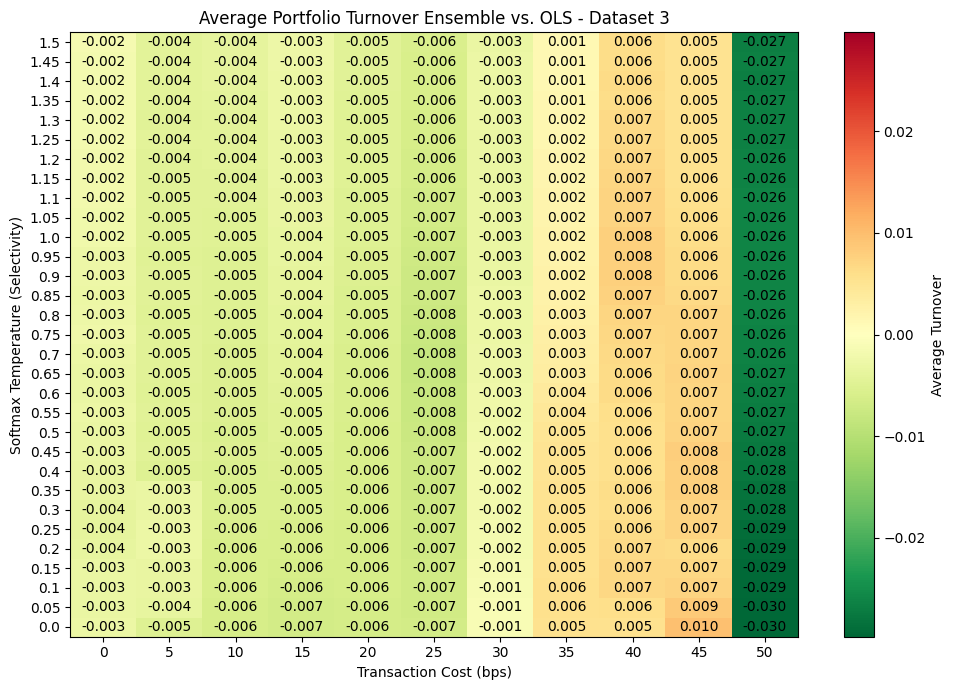
\includegraphics[width=0.75\textwidth]{Turn_ENS_OLS_D3}
\end{figure}

\break

\begin{figure}[h!]
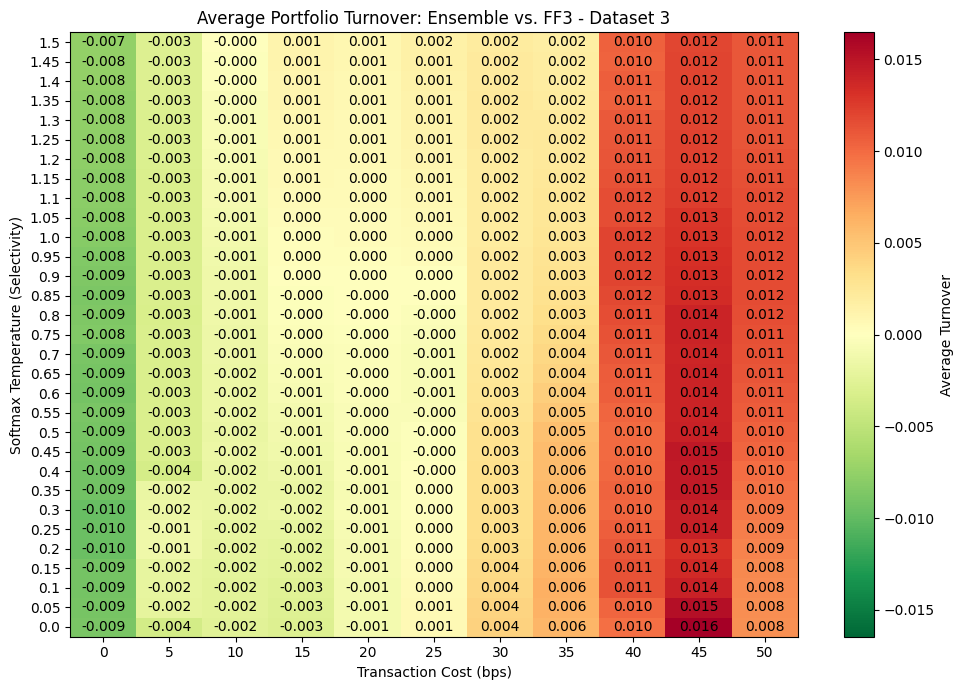
\includegraphics[width=0.75\textwidth]{Turn_ENS_FF3_D3}
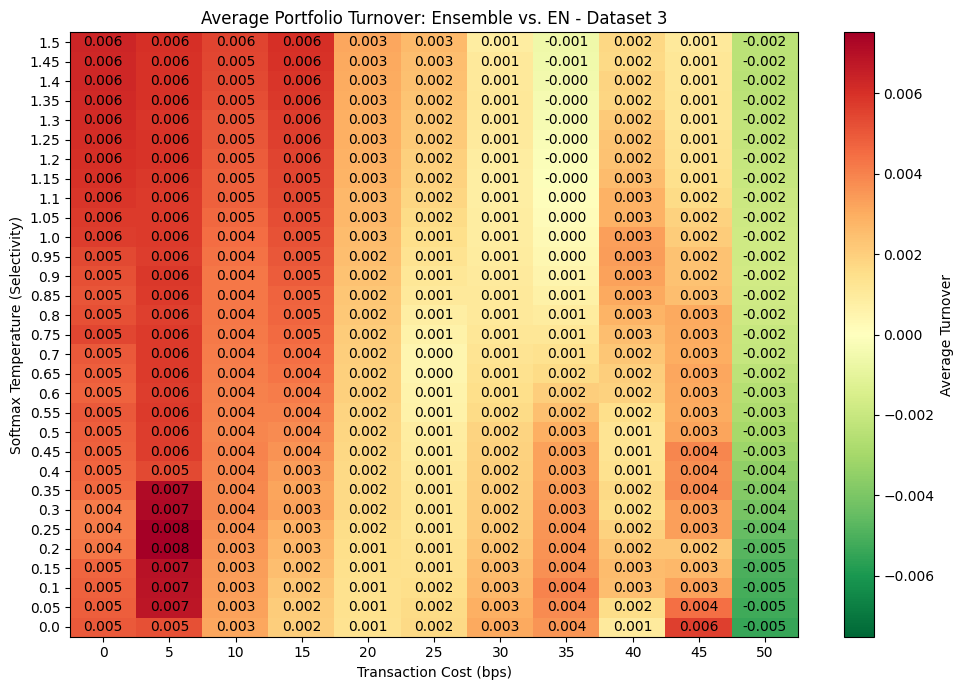
\includegraphics[width=0.75\textwidth]{Turn_ENS_EN_D3}
\end{figure}




\end{document}